\documentclass[10pt]{scrartcl}
\setcapindent{1em}
\addtokomafont{caption}{\small}
\setkomafont{captionlabel}{\sffamily}

\usepackage[a4paper, total={16cm, 24cm}]{geometry}
\usepackage{natbib}
\renewcommand{\bibsection}{\section{\bibname}} \usepackage{authblk}
\renewcommand\Authfont{\Large\sffamily}
\renewcommand\Affilfont{\large}
\author[1]{Nikhil Chandak}
\author[1]{Shashwat Goel}
\author[2]{Dominik Peters}
\affil[1]{IIIT Hyderabad} 
\affil[2]{CNRS, LAMSADE, Universit\'e Paris Dauphine - PSL}
\date{\vspace{-20pt}}

\usepackage[utf8]{inputenc} 

\usepackage[pagebackref]{hyperref}
\hypersetup{
	pdfencoding=auto, 
	psdextra,
	colorlinks=true,
	citecolor=green!50!black,
	linkcolor=red!60!black,
	urlcolor=blue!90!black
}
\renewcommand*{\backref}[1]{[$\to$ p. #1]}


\usepackage{lipsum} \usepackage{multirow} \usepackage{graphicx}
\usepackage{subcaption}
\usepackage{url}            \usepackage{booktabs}       \usepackage{amsmath,amssymb,amsthm}
\usepackage{amsfonts}       \usepackage{nicefrac}       \usepackage{microtype}      \usepackage{xcolor}         \usepackage{enumitem}
\usepackage{float}

\usepackage{wrapfig}
\usepackage{tikz}
\usetikzlibrary{decorations.pathreplacing,calc}
\newcommand{\xmark}{\tikz[scale=0.23,draw=black!50!red] {
    \draw[line width=0.7,line cap=round] (0,0) to [bend left=6] (1,1);
    \draw[line width=0.7,line cap=round] (0.2,0.95) to [bend right=3] (0.8,0.05);
}}
\newcommand{\cmark}{\tikz[scale=0.23,draw=green!50!black] {
    \draw[line width=0.7,line cap=round] (0.25,0) to [bend left=10] (1,1);
    \draw[line width=0.8,line cap=round] (0,0.35) to [bend right=1] (0.23,0);
}}

\usepackage[nameinlink]{cleveref}
\usepackage{crossreftools}
\pdfstringdefDisableCommands{\let\Cref\crtCref
	\let\cref\crtcref
}


\usepackage[vlined,noend]{algorithm2e}


\newcommand*{\alg}{\fontfamily{pcr}\selectfont}

\theoremstyle{plain}
\newtheorem{theorem}{Theorem}[section]
\newtheorem*{theorem*}{Theorem}
\newtheorem{proposition}[theorem]{Proposition}
\newtheorem{lemma}[theorem]{Lemma}
\newtheorem{corollary}[theorem]{Corollary}
\theoremstyle{definition}
\newtheorem{definition}[theorem]{Definition}
\newtheorem{example}[theorem]{Example}
\newtheorem{remark}[theorem]{Remark}
\Crefname{algocf}{Algorithm}{Algorithms}

\usepackage{thmtools}
\usepackage{thm-restate}

\renewcommand*{\le}{\leqslant}
\renewcommand*{\leq}{\leqslant}
\renewcommand*{\ge}{\geqslant}
\renewcommand*{\geq}{\geqslant}
\renewcommand{\epsilon}{\varepsilon}

\newcommand{\alternativea}{\tikz[baseline=-3pt,transform shape,scale=0.85]{\node[text height=6pt,inner sep=1pt,fill=red!20,    circle,minimum width=12pt] (x) {$a$};}}
\newcommand{\alternativeb}{\tikz[baseline=-3pt,transform shape,scale=0.85]{\node[text height=6pt,inner sep=1pt,fill=blue!20,   circle,minimum width=12pt] (x) {$b$};}}
\newcommand{\alternativec}{\tikz[baseline=-3pt,transform shape,scale=0.85]{\node[text height=6pt,inner sep=1pt,fill=green!20,  circle,minimum width=12pt] (x) {$c$};}}
\newcommand{\alternatived}{\tikz[baseline=-3pt,transform shape,scale=0.85]{\node[text height=6pt,inner sep=1pt,fill=orange!20, circle,minimum width=12pt] (x) {$d$};}}
\newcommand{\alternativee}{\tikz[baseline=-3pt,transform shape,scale=0.85]{\node[text height=6pt,inner sep=1pt,fill=magenta!20,circle,minimum width=12pt] (x) {$e$};}}
\newcommand{\alternativef}{\tikz[baseline=-3pt,transform shape,scale=0.85]{\node[text height=6pt,inner sep=1pt,fill=cyan!20,   circle,minimum width=12pt,font=\small] (x) {$f$};}}
\newcommand{\alternativeg}{\tikz[baseline=-3pt,transform shape,scale=0.85]{\node[text height=6pt,inner sep=1pt,fill=brown!20,    circle,minimum width=12pt] (x) {$g$};}}
\newcommand{\alternativeh}{\tikz[baseline=-3pt,transform shape,scale=0.85]{\node[text height=6pt,inner sep=1pt,fill=violet!20,    circle,minimum width=12pt] (x) {$h$};}}

\newcommand{\bigmax}{\mathlarger{\max}}
\newcommand{\bigmin}{\mathlarger{\min}}

\usepackage[backgroundcolor=orange!15!white,bordercolor=orange!80!black,textsize=small]{todonotes}
\tikzset{/tikz/notestyleraw/.append style={rounded corners=0pt,inner sep=0.6ex}}
\presetkeys{todonotes}{inline}{}

\title{Proportional Aggregation of Preferences \\ for Sequential Decision Making}

\usepackage{multicol}
\usepackage{tocloft}

\begin{document}

\newpage
\maketitle

\vspace{-7pt}
\hrule
\vspace{5pt}

\begin{center}
	\textsf{Abstract}
\end{center}

\begin{abstract}
    We study the problem of fair sequential decision making given voter preferences. In each round, a decision rule must choose a decision from a set of alternatives where each voter reports which of these alternatives they approve. Instead of going with the most popular choice in each round, we aim for proportional representation. We formalize this aim using axioms based on Proportional Justified Representation (PJR), which were proposed in the literature on multi-winner voting and were recently adapted to multi-issue decision making. The axioms require that every group of $\alpha\%$ of the voters, if it agrees in every round (i.e., approves a common alternative), then those voters must approve at least $\alpha\%$ of the decisions. A stronger version of the axioms requires that every group of $\alpha\%$ of the voters that agrees in a $\beta$ fraction of rounds must approve $\beta\cdot\alpha\%$ of the decisions. We show that three attractive voting rules satisfy axioms of this style. One of them (Sequential Phragm\'en) makes its decisions online, and the other two satisfy strengthened versions of the axioms but make decisions semi-online (Method of Equal Shares) or fully offline (Proportional Approval Voting). The first two are polynomial-time computable, and the latter is based on an NP-hard optimization, but it admits a polynomial-time local search algorithm that satisfies the same axiomatic properties. We present empirical results about the performance of these rules based on synthetic data and U.S. political elections. We also run experiments where votes are cast by preference models trained on user responses from the moral machine dataset about ethical dilemmas.
\end{abstract}

\vspace{10pt}

\hrule

\vspace{5pt}
{
\setlength\columnsep{17pt}
\setcounter{tocdepth}{2}
\renewcommand\contentsname{\vspace{-20pt}}
\begin{multicols}{2}
	{\footnotesize
	\tableofcontents}
\end{multicols}
}

\vspace{11pt}
\hrule

\newpage

\section{Introduction}
\label{sec:intro}

We consider the problem of making multiple decisions via voting.
In each round, we can choose one alternative from a set of several alternatives, based on voters who tell us which alternatives they support (or \emph{approve}). The set of voters stays the same across rounds, though the set of alternatives may change. 
The simplest way of making these decisions is to take, in each round, the alternative with the most supporters. 

A problem with this method is that non-majority groups of voters may have very little influence on the outcomes. For example, if there is a fixed group of 51\% of the voters who all report the same opinion in every round, then 100\% of the decisions will be taken in accordance with the wishes of that group, with the other 49\% of voters ignored or at most acting as tie-breakers. In many contexts, this will be undesirable, either due to fairness concerns or because the decision maker wishes to hear from each voter to an equal extent.

Following recent work that studies this model under the name ``perpetual voting'' \citep{lackner2020perpetual}, we define formal properties of voting rules that capture the intuition that a group of $\alpha\%$ of the voters should be able to control the decisions in $\alpha\%$ of the rounds. Inspired from work in multi-winner approval voting \citep{lacknerskowron}, we then define a number of voting rules that satisfy these properties. We believe that these rules have promising applications in a variety of domains:

\begin{itemize}[leftmargin=15pt]
	\item \emph{Hiring decisions}: Consider a department hiring new faculty each year, with existing faculty voting over the applicants. The department wishes to hire people representing its spectrum of research interests. For example, if 20\% of the department works on one topic and votes for candidate on that topic, then at least 1 such candidate should be hired every 5 years.
	\item \emph{Uncertainty about the goal}: Suppose we are managing an intelligent system that is repeatedly deciding on an action in order to maximize an objective function that we have specified. But we may not be certain about our desired objective function (for example because we have \emph{moral uncertainty}). Literature in reinforcement learning explores similar problems like \emph{reward uncertainty} \citep{liang2022reward} and in the \emph{cooperative IRL framework} \citep{hadfield2016cooperative}.
    We can decide on a mixture of objectives (20\% on objective 1, etc.). Each objective generates recommendations for good actions in each round, and we can make the decision using our voting rules. 
	\item \emph{Virtual democracy}: In cases where a group of people need to make very many similar decisions, we may wish to automate this process. An approach known as virtual democracy does this by initially learning voters' preferences over a space of potential alternatives (specified by feature vectors) for example based on pairwise comparisons. Then, each decision is made by letting the models vote on the decision maker's behalf by predicting their preferences. This approach has led to proof-of-concept systems that automate moral decisions faced by autonomous vehicles \citep{noothigattu2018voting}, kidney exchanges \citep{freedman2020adapting}, collective decision making directly from natural language preferences \citep{mohsin2021making} and allocation of food donations \citep{lee2019webuildai}. The approach behind these systems has recently been criticized as overweighting the opinions of majorities \citep{moralmachinetyranny}. We show preliminary evidence in our experiments that using proportional voting methods could avoid this issue.
\item \emph{Policy decisions of coalition governments}: In many countries, the government is formed by coalitions of several parties with different strengths (for example, in Germany 2021--25 it consists of 3 parties who received 26\%, 15\%, and 12\% of the vote). A coalition needs to agree on a program, consisting of decisions on many issues. Our methods could help to design a program where each party's influence is proportional to their vote strength.
	\item \emph{Combining generative models}: More speculatively, one could use these methods to ``mix'' different generative models such as large language models that produce a sequence of tokens one by one. Recently introduced models such as chatGPT, Bing Chat, Bard, and others have different styles, personalities, and strengths, and it is common for users to query several models at once. Instead, one could let users specify a desired mixture of these models, and produce the output sequence by letting the models vote on the next token. On a related note, \citet{bakker2022fine} have recently used LLMs to generate consensus statements that maximize expected approval for a group of people with diverse opinions. Given that they collect data for the group over several issues, our methods can be used in such cases to produce proportional outcomes. 
\end{itemize}

\paragraph{Our results}

\begin{table}
	\centering
	\newcommand{\ejrremark}{\raisebox{0.9pt}{*}\hspace{-5pt}}
	\begin{tabular}{llcccc}
		\toprule
		& Best known voting rule & \:PJR\: & Strong PJR & \:\:EJR\:\: & Strong EJR \\
		\midrule
		Online & Sequential Phragm\'en & \cmark & \cmark & \xmark\ejrremark{} & \xmark\ejrremark{} \\
		Semi-online & Method of Equal Shares & \cmark &  \xmark & \cmark& \xmark \\
		Offline & PAV & \cmark & \cmark & \cmark & \cmark \\
		\bottomrule
	\end{tabular}
	\vspace{5pt}
	\caption{Our results. For each setting (online, semi-online (where the rule knows the total number of rounds in advance), offline (where the rule knows all the preferences in advance)), we list the best known rule with respect to proportionality axioms. * = knowing an online rule satisfying EJR (or Strong EJR) would resolve an open problem in the theory of multi-winner approval voting.}
	\label{tab:results}
\end{table}

We build on the work of \citet{bulteau2021jr} who defined axioms that guarantee group representation. We consider two of them, which we will call PJR (Proportional Justified Representation) and Strong PJR. \citet{bulteau2021jr} gave existence proofs showing that for every possible voting input, there exists an output satisfying both axioms, though their proofs do not suggest a natural voting rule or even a polynomial-time algorithm. In fact, \citet{bulteau2021jr} conjecture that no polynomial-time algorithm can find a PJR outcome. We show that the picture is more positive: an attractive polynomial-time voting rule building on ideas of \citet{Phra94a} satisfies Strong PJR (\Cref{sec:guarantees:phragmen}). This rule is fully online, making decisions round by round.

We then define an axiom called EJR (Extended Justified Representation), which provides better group representation guarantees than PJR. 
We define a simple voting rule (a variant of the ``Method of Equal Shares'') that satisfies EJR which is ``semi-online'': it needs to know how many rounds there will be in total, but it can be given preferences in an online fashion (\Cref{sec:guarantees:mes}).  
However, the Method of Equal Shares does not satisfy Strong PJR.
A rule that maximizes a carefully chosen objective function proposed by \citet{Thie95a} known as Proportional Approval Voting (PAV) does satisfy EJR and Strong PJR, and even satisfies a new axiom that we define called Strong EJR (\Cref{sec:guarantees:pav}). While the PAV optimization problem is NP-hard, we prove that a polynomial-time local search variant of the rule also satisfies Strong EJR. However, PAV is an offline rule and needs to know full preference information for all the rounds in advance. We do not know an online rule satisfying EJR or Strong EJR, and we show (in the appendix) that finding such a rule would resolve a major open problem in the literature on multi-winner approval voting \citep{lacknerskowron}.

We also consider several different ways of defining stronger axioms than (Strong) PJR and EJR, which either give groups better utility guarantees or give guarantees to more groups. However, by giving counterexamples, we show that these strengthenings are not always satisfiable (\Cref{sec:hardness}).

We close with several simulations that compare our rules to existing rules from the literature (which do not give group fairness guarantees). 
These simulations are based on synthetic data (where we randomly generate approvals in such a way that there are a small number of distinct cohesive voter groups) and on U.S. political election data (\Cref{sec:experiments:synthetic,sec:experiments:political}).
We also run an experiment for the \emph{virtual democracy} application. Following \citet{noothigattu2018voting}, we use the \emph{moral machine} dataset \citet{awad2018moral}, containing several million ethical judgments by respondents from around the world about how a self-driving car should behave in trolley-problem-style dilemmas. We partition the responses according to the country of the respondent. For each country, we learn a preference model predicting the judgments of respondents from the country. We treat each country as a `voter'. We then sample new decision situations and query the models for the ethically best decisions in that situation, and aggregate the responses using our voting rule. We compare the aggregated response to an alternative approach where a single model is trained based on responses from all countries (with each country contributing the same number of data points for balance). Based on our metrics, we find that the aggregation approach leads to a fairer outcome, in the sense that agreement with the decision is more equally distributed across countries, compared to the decision made by the combined model (\Cref{sec:experiments:learning}).



 \newpage
\section{Related Work}
\label{sec:related}

\paragraph{Perpetual Voting}
Our work is most closely related to perpetual voting \citep{lackner2020perpetual} which concerns online sequential decision making based on approval votes. In this paper, we also consider offline rules. \citet{lackner2020perpetual} focussed on \emph{individual} fairness properties, for example requiring that each voter approves at least 1 decision in every time interval of some bounded length. We are interested in guarantees for \emph{groups} of voters who agree with each other, such that larger groups receive stronger guarantees. Such guarantees have been considered by \citet{lacknermaly2023} and \citet{bulteau2021jr}; we compare them to ours in \Cref{sec:formulation}. \citet{lacknermaly2023} also consider ``upper quota'' axioms, which require that groups are not overrepresented in the outcome; we only consider axioms that prevent underrepresentation.

\paragraph{Public Decision Making}
\citet{fairpublicdecisionmaking} proposed a model they call ``public decision making'' which is an offline model of several decisions, where voters have a utility value for each alternative in each round, and a voter's total utility is the sum of the utilities obtained in each round. We study the special case where the utility values are restricted to 0 and 1. \citet{fairpublicdecisionmaking} focus on fairness notions for individuals (not groups) derived from ideas in fair division. \citet{freeman2017fairdynamic} study an online version of this setting.
\citet{freeman2020proportionality} and \citet{skowron2022proportionalpublicdecisions} consider the special case where there are exactly two alternatives (``yes/no'') in each round and utilities are 0/1, which is a simple special case of our setting where fairness properties are easier to obtain. \citet{propinterdependentissues} consider the same setting with interdependent issues.

\paragraph{Repeated Portioning}
In our model, we need to choose one alternative in each round. One could define a fractional version of this model, where in each round, we choose a \emph{mixture} of the available alternatives (formally, a probability distribution or lottery over $C_j$). In the single-round setting, finding a fair mixture has been considered by several papers \citep{BMS05a,FGM16a,ABM20a,BBPS21a}. For a multi-round setting with online decisions, this model is studied by \citet[Section 5]{banerjee2023proportionally} who consider a proportional fairness objective and propose methods with good regret bounds. 

\paragraph{Multi-winner Approval Voting} 
For the task of selecting a committee of exactly $k$ out of $m$ candidates given approval votes \citep{lacknerskowron}, proportionality has been intensely studied. Many axioms have been proposed that formalize the idea that $\alpha\%$ of the voters should be able to elect at least $\alpha\% \cdot k$ of the committee members \citep{ejr,pjr,PeSk20,ejr+}. Voting rules proposed long ago by \citet{Thie95a} and \citet{Phra94a} do very well with respect to these axioms \citep{Jans16a,brill2023phragmen}. A more recent rule proposed by \citet{PeSk20} known as the Method of Equal Shares combines some of the advantages of the Phragmén and Thiele rules. \citet{skowron2017proportional} discuss adapting multi-winner rules to obtain ``proportional rankings'' of alternatives, which can be seen as a sequential decision making problem. Many of the rules and axioms we consider in this paper are analogues or generalizations of proposals from multi-winner voting. 

\paragraph{Approval-based Apportionment}
\citet{approvalbasedapportionment} considered a model where we need to assign $k$ seats to political parties, based on voters who submit approval sets over parties. This can be seen as a kind of multi-winner election where candidates can be added to the committee several times (because a single party can receive multiple seats). Alternatively, it can be seen as a special case of our model with $k$ rounds, where the sets of alternatives and all voters' approval sets remain the same across all rounds. Being a special case of our model, some negative results of \citet{approvalbasedapportionment} carry over to our model, notably that Sequential Phragm\'en fails EJR and that PAV is NP-hard to compute; we will mention these connections during our discussion.

\paragraph{Combinatorial Voting}
A classic literature on voting in combinatorial domains \citep{LaXi15a} studies the problem of making decisions on several issues. The main focus is on the representation of complex preferences (where preferences on one issue may be conditional on the decision in other issues), and the computational problem of finding good outcomes given such preferences, often in the sense of maximizing utilitarian or egalitarian welfare \citep{amanatidis2015multiple}. Some of this work considers (conditional) approval preferences \citep{barrot2016conditional}. \newpage
\section{Problem Formulation}
\label{sec:formulation}


\subsection{Model}

Let $N = \{1, 2, \ldots, n\}$ be the set of \emph{voters}, with $|N|=n$. There is a set $R = \{1, 2, \dots, T \}$ of $T$ \emph{rounds}, where $T$ is the \emph{time horizon}. 
In each round $j\in R$, we are given a set of \emph{alternatives} $C_j$. 
Each voter $i \in N$ \emph{approves} some subset $\smash{A^i_j}$ of $C_j$. 
Thus, we have a sequence of $T$ decision rounds together with a sequence $C = (C_j)_j$ of alternative sets and a collection $A = (A^i_j)_{i\in N, j})$ of approval sets.
We call the quadruple $(N, R, C, A)$ a \emph{decision instance}. 

A \emph{decision sequence} $D = (d_1, \dots, d_T) \in C_1 \times \dots \times C_T$ specifies a single \emph{decision} $d_j \in C_j$ for each round $j \in R$. For a voter $i \in N$, we write $\smash{U^i_D = |\{ j \in R : d_j \in A^i_j \}|}$ for the number of decisions in $D$ that $i$ approves; we treat $U^i_D$ as $i$'s \emph{utility}. 
A \emph{decision rule} $f$ takes as input a decision instance and returns a decisions sequence $D = f(N, R, (C_j)_{j}, (A^i_j)_{i\in N, j})$. We call a decision rule \emph{semi-online} if its decision in round $j \in R$ only depends on the information up to round $j$, i.e., on $N$, $R$, $C_1, \dots, C_j$ and $\smash{A_1^i, \dots, A_j^i}$. A rule is \emph{online} if in addition, the decision in round $j$ does not depend on the time horizon $T$. 




\subsection{Axioms}
\label{sec:axioms}

\begin{wrapfigure}[17]{r}{7.2cm}
	\vspace{-13pt}
	\centering
	\scalebox{0.84}{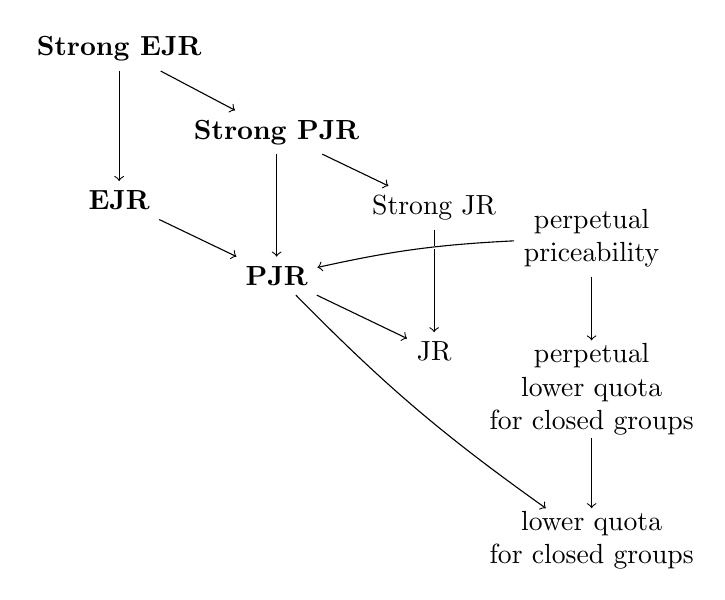
\begin{tikzpicture}[yscale=0.96]
			\node at (0,5) (strongEJR) {\textbf{Strong EJR}};
			\node at (0,3) (EJR) {\textbf{EJR}};
			
			\node at (2,3.9) (strongPJR) {\textbf{Strong PJR}};
			\node at (2,2) (PJR) {\textbf{PJR}};
			
			\node at (4,2.9) (strongJR) {Strong JR};
			\node at (4,1) (JR) {JR};
			
			\node[align=center] at (6,2.5) (price) {perpetual\\priceability};
			\node[align=center, inner sep=1pt] at (6,0.5) (plq) {perpetual \\ lower quota \\ for closed groups};
			\node[align=center, inner sep=1pt] at (6,-1.5) (lq) {lower quota \\ for closed groups};
			
			\draw[->] 
			(strongEJR) edge (EJR) 
			edge (strongPJR)
			(strongPJR) edge (strongJR)
			edge (PJR)
			(strongJR) edge (JR)
			(EJR)		edge (PJR)
			(price)		edge (plq)
			(plq)         edge (lq)
			(PJR)		edge[bend right=5] (lq)
			edge (JR);
			
			\fill[white] (3.5, 2.4) rectangle (4.5, 2.36); 

			\draw[->] (price) edge[bend right=5] (PJR);
	\end{tikzpicture}}
	\vspace{-12pt}
	\caption{Implications between axioms. We focus on the axioms in bold.}
	\label{fig:hasse}
\end{wrapfigure}

We now define several properties (or \emph{axioms}) of decision sequences that formalize the idea of proportional representation. These come in different strengths and \Cref{fig:hasse} shows implication relationships between them. We will focus on the four strongest properties of (Strong) EJR and (Strong) PJR. For completeness, we also mention two other properties introduced by \citet{lacknermaly2023}: we discuss \emph{lower quota for closed groups} in \Cref{app:closed-groups} and \emph{perpetual priceability} in \Cref{app:priceability}. In \Cref{app:pareto}, we briefly discuss Pareto efficiency.

Our first two main axioms were introduced by \citet{bulteau2021jr}.\footnote{We use different names for these axioms. \citet{bulteau2021jr} use the term ``all periods intersection PJR'' for what we just call PJR, and the term ``some periods intersection PJR'' for what we call Strong PJR.}
Let us say that a group $S\subseteq N$ of voters \textit{agrees} in round $j \in R$ if there is an alternative $c \in C_j$ that all voters in $S$ approve, so $\bigcap_{i\in S} A^i_j \neq \emptyset$. PJR (short for Proportional Justified Representation) requires that a group of an $\alpha$ fraction of the voters, if they agree in every round, must be ``happy'' with at least an $\alpha$ fraction of the decisions. We define this to mean that in $\lfloor \alpha T \rfloor$ many rounds, at least one member of $S$ approves the decision (but this member of $S$ can be different in each round).

\begin{definition}[PJR]
    \label{def:PJR}
    A decision sequence $D$ satisfies \emph{PJR} if for every $\ell \in \mathbb N$ and every group of voters $S \subseteq N$ that agrees in every round and has size $|S| \geq \ell \cdot \frac{n}{T}$, there are at least $\ell$ rounds $j \in R$ in which the decision $d_j$ of $D$ is approved by at least one voter in $S$ (i.e., $d_j \in \bigcup_{i \in S} \smash{A_j^i}$).
\end{definition}

PJR only provides guarantees for groups that agree in \emph{all} rounds. Strong PJR also gives guarantees for groups that agree only in some of the rounds, though the groups need to be larger: a group that agrees in $k$ rounds deserves to be happy with $\ell$ decisions if the size of the group is at least $\ell \cdot \frac{n}{k}$ (as compared to $\ell \cdot \frac{n}{T}$ for groups that agree in all rounds). Note that Strong PJR implies PJR (take $k = T$).

\begin{definition}[Strong PJR]
    \label{def:strongPJR}
    A decision sequence $D$ satisfies \emph{Strong PJR} if for every $\ell \in \mathbb N$ and every group of voters $S \subseteq N$ that agrees in $k$ rounds and has size $|S| \geq \ell \cdot \frac{n}{k}$, there are at least $\ell$ rounds $j \in R$ in which the decision $d_j$ of $D$ is approved by at least one voter in $S$ (i.e., $d_j \in \bigcup_{i \in S} \smash{A_j^i}$).
\end{definition}

An equivalent way of stating this axiom is that an $\alpha$ fraction of the voters who agree in a $\beta$ fraction of the rounds need to be ``happy'' with at least an $\lfloor \alpha \cdot \beta \rfloor$ fraction of the decisions. For example, consider a group $S\subseteq N$ of voters with fixed size $\ell \cdot \frac{n}{T}$, and let us ask what Strong PJR guarantees for this group. If $S$ agrees in all rounds, then it says that $S$ should be happy with $\ell$ decisions. If $S$ agrees in $\frac{T}{2}$ rounds, then it says that $S$ should be happy with $\lfloor \frac{\ell}{2}\rfloor$ decisions. Thus, the guarantee provided to a group is proportional to the number of rounds in which the group agrees.

Following the literature on multi-winner voting, we say that a decision sequence satisfies (Strong) \emph{JR} (Justified Representation) if it satisfies (Strong) PJR restricted to $\ell = 1$. Several of our counterexamples will apply even to JR and to Strong JR.

To illustrate the axioms, consider the instance shown in \Cref{fig:axiom-example}, with $T = 8$ rounds and 4 voters. The first two voters form a group $S = \{1,2\}$ that agrees in all rounds (because they both always approve $\alternativea$). Thus, for an outcome to satisfy PJR, in at least $\ell = 4$ rounds the outcome needs to be either $\alternativea$, $\alternativeb$, or $\alternativec$ (because $|S| \ge \ell \cdot \frac48$). The group $S' = \{3, 4\}$ agrees in the first 6 rounds (approving $\alternatived$), so with $\ell' = 3$, because $|S'| \ge \ell' \cdot \frac{4}{6}$, Strong PJR requires that in at least $3$ rounds, the outcome is either $\alternatived$, $\alternativee$, or $\alternativef$.

\begin{wrapfigure}[9]{r}{7.1cm}
	\vspace{-3pt}	
	\centering
	\scalebox{0.9}{\setlength{\tabcolsep}{4pt}
		\begin{tabular}{lcccccccc}
			\toprule
			Round & 1 \& 2 & 3 \& 4 & 5 \& 6 & 7 \& 8 \\
			\midrule
			Voter 1 & $\{\alternativea, \alternativeb\}$ & $\{\alternativea, \alternativeb\}$ & $\{\alternativea, \alternativeb\}$ & $\{\alternativea, \alternativeb\}$ \\
			Voter 2 & $\{\alternativea, \alternativec\}$ & $\{\alternativea, \alternativec\}$ & $\{\alternativea, \alternativec\}$ & $\{\alternativea, \alternativec\}$ \\
			Voter 3 & $\{\alternatived\}$ & $\{\alternatived\}$ & $\{\alternatived\}$ & $\{\alternativee\}$ \\
			Voter 4 & $\{\alternatived\}$ & $\{\alternatived\}$ & $\{\alternatived\}$ & $\{\alternativef\}$ \\
			\bottomrule
	\end{tabular}}
	\caption{Example illustrating our axioms.}
	\label{fig:axiom-example}
\end{wrapfigure}






A weakness of PJR and Strong PJR is in how they define $S$ being ``happy'' with a decision (``at least one member of $S$ approves the decision''). This definition could be satisfied by a decision sequence that gives each member of $S$ a utility that is much lower than $\ell$ \citep[Sec.~4.2]{PeSk20}. In the example of \Cref{fig:axiom-example}, the decision sequence $(\alternativeb,\alternativeb,\alternativec,\alternativec,\alternatived,\alternatived,\alternativee,\alternativef)$ satisfies Strong PJR, but the first two voters each only approve the decision in 2 rounds, instead of in 4 rounds. 
Following \citet{ejr}, we can fix this issue by defining the axioms EJR (short for Extended Justified Representation) and Strong EJR. These axioms require that at least one member $i$ of $S$ must approve at least $\ell$ of the decisions, i.e., must have utility $\smash{U^i_D} \ge \ell$. In the example, the decision sequence $(\alternatived,\alternatived,\alternatived,\alternatived,\alternativea,\alternativea,\alternativea,\alternativea)$ satisfies Strong EJR.

\begin{definition}[EJR]
    \label{def:EJR}
    A decision sequence $D$ satisfies \emph{EJR} if for every $\ell \in \mathbb N$ and every group of voters $S \subseteq N$ that agrees in all rounds and that has size $|S| \geq \ell \frac{n}{T}$, there exists a voter $i\in S$ who approves at least $\ell$ decisions in $D$, i.e., $\smash{U^i_D} \ge \ell$.
\end{definition}

\begin{definition}[Strong EJR]
    \label{def:strongEJR}
    A decision sequence $D$ satisfies \emph{Strong EJR} if  for every $\ell \in \mathbb N$ and every group of voters $S \subseteq N$ that agrees in $k$ rounds and has size $|S| \geq \ell \cdot \frac{n}{k}$, there exists a voter $i \in S$ who approves at least $\ell$ decisions in $D$, i.e., $\smash{U^i_D} \ge \ell$.
\end{definition}

A decision rule $f$ \emph{satisfies} one of these axioms if for all possible inputs, the decision sequence selected by $f$ satisfies it. Note that if $f$ is also online, this means that the proportionality guarantee thereby not only holds for the entire decision sequence, but also for every prefix of it.

\subsection{Methods}

We now define three decision rules that are natural analogues of rules that were first proposed in the context of multi-winner elections.

\subsubsection{Sequential Phragm\'en}
\citet{Phra94a} proposed an approval-based voting method for electing members of the Swedish parliament. \citet{lacknermaly2023} adapted this rule to the context of perpetual voting, calling their adaptation ``perpetual Phragm\'en''. We follow their definition. The rule makes decisions round by round. Its main idea is that each decision provides a value of 1, and this value (usually referred to as \emph{load}) will be distributed to the voters who approve the decision. In each round, the rule chooses an alternative such that no voter ends up with too much load, thereby prioritizing voters who do not yet agree with many prior decisions. Formally, each voter $i$ starts with load $x^i=0$. Sequential Phragm\'en chooses the alternative for which it can distribute a load of $1$ in a way that minimizes the maximum total load assigned to a voter: at each round $j \in R$, we compute the following value for each alternative $c \in C_j$: 
\[ s_c = \min_{S \subseteq \{ i \in N : c \in A^i_j \}}  \frac{\sum_{i \in S} x^i + 1}{|S|}.\] 
\begin{wrapfigure}[5]{r}{4.4cm}
	\vspace{-66pt}
	\centering
	\scalebox{0.96}{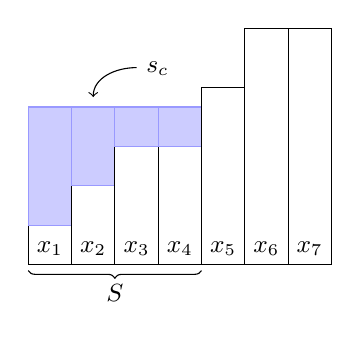
\begin{tikzpicture}
		[xscale=0.55, yscale=0.5, font=\small,
		bracepath/.style={decorate, decoration = {brace, mirror, transform={yscale=1.1,yshift=-2pt}}},]
		\foreach 
			\voter/\load/\newload
			in {1/1/3,2/2/2,3/3/1,4/3/1,5/4.5/0,6/6/0,7/6/0}
			{
\draw (\voter-1,0) rectangle (\voter,\load);
\ifnum\newload>0
					\draw[blue!40, fill=blue!20] (\voter-1,\load) rectangle (\voter,\load+\newload);
				\fi
				\node at (\voter-0.5,0.4) {$x_\voter$};
			}
			
\draw[out=180, in=90, ->] (2.5,5) to (1.5,4.25);
		\node[anchor=west] at (2.5,4.97) {$s_c$};
			
\draw[bracepath] (0,0) -- (4,0);
		\node[anchor=north] at (2,-0.25) {$S$};
	\end{tikzpicture}}
	\vspace{-7pt}
	\caption{Load distribution}
	\label{fig:load}
\end{wrapfigure}
This value can be understood using a ``water filling'' analogy, as shown in \Cref{fig:load}, where we consider an alternative $c$ approved by 7 voters, and show their current loads as bars. We then fill 1 unit of blue water on top of the approving voters' loads. Note that the water never falls on top of the loads of voters $5$, $6$, and $7$ because their load is already quite high; in other words, this process has only assigned load to the set $S = \{1,2,3,4\}$. Then $s_c$ is the ``water line'', which is the load of each voter in $S$ after the load of $c$ has been assigned.

The decision for round $j \in R$ is the alternative $c$ that minimizes $s_c$, breaking ties arbitrarily. After making the decision, we update loads by setting $x^i = s_c$ for each voter $i \in S$ (where $S$ is the coalition attaining the minimum in the definition of $s_c$) and leave $x^i$ unchanged for voters not in $S$. 
Note that the load of a voter will never decrease.\footnote{In the multi-winner setting, it is not necessary to define $s_c$ using a minimization over $S$, and we can just take $S$ to be the set of \emph{all} voters approving $c$. This is because in multi-winner voting, it cannot happen that an approver of $c$ already has more load than $s_c$, because in that case the rule would have chosen $c$ in an earlier iteration \citep[Lemma 4.5]{brill2023phragmen}. This argument does not work in our setting because $c$ may not have been available in a prior round. An alternative definition of Phragm\'en's method in multi-winner voting is based on virtual bank accounts that are continuously filled \citep{Jans16a,PeSk20}. This definition does not easily adapt to our setting due to a similar problem: if in some round no good alternative exists, then the bank accounts will fill up too much, leading to ties in later rounds.}
Clearly, Sequential Phragm\'en is an online rule that requires no information about future rounds. \citet{lacknermaly2023} show that it can be computed in polynomial time, and provide a detailed example of how the rule works.

\subsubsection{Method of Equal Shares (MES)}
MES is a recently introduced voting rule for multi-winner voting \citep{PeSk20} and participatory budgeting \citep{peters2021proportional}. It can be adapted to our setting in a semi-online fashion: the rule needs to know the total number of rounds $T$ in advance, but does not need to know voter preferences of future rounds. MES makes decisions round by round. Similar to the concept of load in Sequential Phragm\'en, each decision costs $p=\frac{n}{T}$ units which must be distributed among voters who approve the alternative. MES works by subtracting this amount from an initial budget assigned to each voter. Formally, let $b^i = 1$ be the initial budget of voter $i$. 
For $\rho \ge 0$, we say that an alternative $c \in C_j$ is $\rho$-\emph{affordable} if $\smash{\sum_{i \in N : c \in A^i_j} \min(b^i, \rho)} \geq p$ (so approvers of $c$ can pay the amount $p$ with their remaining budgets even if no one pays more than $\rho$). 
In each round, the alternative $d_j \in C_j$ that is $\rho$-affordable for minimum $\rho$ is chosen, breaking ties arbitrarily. Then for each voter $i$ approving $d_j$, $i$'s remaining budget $b^i$ is set to $\max(0, b^i - \rho)$.
If in some round $j \in R$, no alternative can be bought for any $\rho$, i.e., $\smash{\sum_{i \in N : c \in A^i_j} b^i} < p$ for all alternatives $c \in C_j$, MES \emph{terminates prematurely}. For purposes of our theoretical results, it does not matter how the decisions for remaining rounds are made. All these results (positive and negative) hold for every way of completing the partial decision sequence that is output by MES. 

For actual implementations of MES, one can choose between several ``completion rules'', which are familiar from work on multi-winner voting and participatory budgeting. In our experiments, we followed the ``$\epsilon$-completion'' strategy introduced by \cite[Sec.~3.4]{peters2021proportional}. In a round $j \in R$ where no alternative is affordable according to the definition of MES,
we will choose an alternative $a_j \in C_j$ and make all voters who approve $a_j$ spend all their remaining money to cover as much cost $p$ of the round as possible. The remaining part of the cost is covered by the voters $i\in N$ who don't approve $a$ so that the maximal payment of such a voter, $\gamma$, is minimized. We select the alternative $a_j \in C_j$ minimizing $\gamma$ and update voters' individual budgets.



It is also possible to run MES in an offline fashion (``Offline MES''), by letting it choose at each step in which round it would like to make a decision (namely, the round where some alternative is $\rho$-affordable for minimal $\rho$, across all alternatives in all rounds where no decision has been taken yet). All our proofs and counterexamples go through for Offline MES, so it also satisfies EJR but fails Strong PJR.

\enlargethispage{10pt}
\subsubsection{Proportional Approval Voting (PAV)}
\citet{Thie95a} proposed an alternative method to Phragm\'en's, which is based on optimizing an objective function. We adapt this method to our context in an offline way. PAV selects the decision sequence $D \in C_1 \times \dots \times C_T$ that maximizes
\[
\operatorname{PAV-score}(D) = \sum_{i\in N} 1 + \frac12 + \frac13 + \dots + \frac1{U^i_D},
\] 
where we recall that $U^i_D$ is the number of rounds in which voter $i$ approves the decision of $D$. This harmonic objective function is the unique additive objective that leads to a proportional rule \citep{ejr}.
Finding the optimum decision sequence for PAV is NP-hard \citep[Thm.~5.1]{approvalbasedapportionment}, just like in the multi-winner setting \citep{aziz2015computational}, but we will show that a polynomial-time local search variant \citep{aziz2018complexity} satisfies the same axioms as PAV.\footnote{There also exists a sequential version of PAV that could be applied to our setting to give an online rule. Based on simulations, \citet{page2020electingexecutive} conjecture that this rule would satisfy at least a weak version of PJR. However, a result of \citet[Footnote 4]{approvalbasedapportionment} implies that the sequential version fails this property.}
 \section{Satisfying the Axioms}
\label{sec:guarantees}

In this section, we establish which of our three rules satisfy which of our four axioms (see \Cref{tab:results}).
\citet{bulteau2021jr} conjectured that no polynomial-time rule achieves PJR (their existence proof were based on an exponential algorithm). Our results show that in fact, PJR as well as the stronger axioms can be satisfied in polynomial time, by attractive rules, some of which even work online.

\subsection{Online: Sequential Phragm\'en}
\label{sec:guarantees:phragmen}

We begin by analyzing the sequential Phragm\'en rule. 
\begin{theorem}
    Sequential Phragm\'en satisfies Strong PJR.
\end{theorem}

\begin{proof}
For a contradiction, suppose that $S \subseteq N$ witnesses a violation of Strong PJR: it agree in the set of rounds $R^* = \{j_1, \dots, j_k\} \subseteq R$ and has size $|S| \ge \ell \cdot \frac{n}{k}$, but there are fewer than $\ell$ rounds in which at least one member of $S$ approves the decision.

First, we claim that if $d_j \in C_j$ is the alternative chosen in some round $j \in R^*$, then $s_{d_j} \leq \frac{\ell }{|S|}$. Note that the total load $\sum_{i \in S} x^i$ assigned to members of $S$ is at most $\ell - 1$ because each decision incurs a load of 1. Since $j\in R^*$, there is an alternative $c' \in C_j$ that everyone in $S$ approves. Hence, 
\[
s_{c'} \leq \frac{1 + \sum_{i \in S}x^i}{|S|} \leq \frac{1 + (\ell-1)}{|S|} = \frac{\ell}{|S|},
\]
where the first inequality follows from the definition of $s_{c'}$ as a minimum. Since Sequential Phragm\'en selected $d_j$, we have $s_{d_j} \le s_{c'}$, showing our claim.

Call a round $j \in R^*$ a \emph{bad round} if the decision $d_j$ is not approved by any voter in $S$.
Now let $i \in N \setminus S$ be a voter not in $S$, and suppose $i$ gets assigned some load during at least one bad round. Consider the point just after the last bad round where $i$ is assigned some load. 
At this point we must have $x^i \le \frac{\ell }{|S|}$ because otherwise $s_{d_j} > \frac{\ell }{|S|}$, contradicting our previous claim. 
Thus, at most $\frac{\ell }{|S|}$ load was assigned to $i$ during bad rounds (i.e., adding up the load additions to $i$ over all bad rounds). 
Clearly, this last claim is also true for voters $i \in N \setminus S$ who do not get assigned any load during any bad round.

In a bad round, load is only assigned to voters outside $S$ (since the round is bad). Thus, we can now bound the total load that gets assigned in bad rounds, by summing over all $i \in N\setminus S$; it is at most
\[
\textstyle
|N \setminus S| \cdot  \frac{\ell}{|S|}  = \frac{|N|}{|S|}\cdot \ell - \frac{|S|}{|S|}\cdot \ell \leq \frac{k}{\ell}\ell - \ell = k - \ell.
\]
However, there are at least $k - (\ell - 1)$ bad rounds, so a total load of at least $k - \ell + 1$ is distributed across bad rounds, a contradiction.
\end{proof}

In multi-winner voting, Sequential Phragm\'en is well-known to fail EJR \citep{brill2023phragmen}, so it is unsurprising that it also fails EJR in our setting. While it is possible to adapt the example of \citet{brill2023phragmen} to our setting, we use a somewhat simpler example.\footnote{This example can also be used to show that Sequential Phragm\'en fails EJR for the related settings of approval-based apportionment and of multi-winner voting. We thus add a different EJR counterexample to the literature, which may turn out useful in future work.}

\begin{theorem}
    Sequential Phragm\'en fails EJR.
\label{thm:phragmen_fails_EJR}
\end{theorem}

\begin{wrapfigure}[10]{r}{5.8cm}
	\vspace{-12pt}	
	\centering
	\scalebox{0.94}
	{\setlength{\tabcolsep}{4pt}
		\begin{tabular}{lccc}
			\toprule
			Rounds & 1 \ - \ 10 \\
			\midrule
			Voters 1, 2, 3 & $\{\alternativea, \alternativeb\}$ \\
			Voters 4, 5, 6, 7  & $\{\alternativea, \alternativec\}$  \\
			Voters 8, 9  & $\{\alternativeb, \alternativec\}$ \\
			Voter 10 & $\{\alternativeb\}$  \\
			\bottomrule
	\end{tabular}}
	\caption{Instance where Sequential Phragm\'en fails EJR. Note that the approval sets are the same in all rounds.}
	\label{fig:phragmen_fails_EJR_simpler_example}
\end{wrapfigure}

\noindent
\emph{Proof.}\: Consider the instance shown in \Cref{fig:phragmen_fails_EJR_simpler_example}, with $T = 10$ rounds and $n = 10$ voters. Here, the same profile is repeated for the all the rounds, so it is also an example where Sequential Phragm\'en fails EJR in the setting of approval-based apportionment \citep{approvalbasedapportionment}. In this example, Sequential Phragm\'en alternates between two alternatives as winner in each round and produces the decision sequence $D = (\alternativea, \alternativeb, \alternativea,\alternativeb, \alternativea, \alternativeb, \alternativea, \alternativeb, \alternativea, \alternativeb\} $. The first three voters approve all the decisions of the outcome, so each of them gets a satisfaction of $10$ while the rest of the voters approve only half of the decisions from $D$, so they each get a satisfaction of $5$.  The coalition $S = \{4, 5, 6, 7, 8, 9\}$ agrees in all rounds on $\alternativec$, so EJR demands that at least one voter in $S$ should approve at least $\ell = 6$ decisions (since $6 = |S| \ge \ell \cdot \frac{n}{T} = 6 \cdot \frac{10}{10}$). However, each voter in $S$ approves the decision of only $5$ rounds, which is strictly less than $\ell = 6$, so EJR is violated. Hence, Sequential Phragm\'en fails EJR. \hfill\qed


\subsection{Semi-online: Method of Equal Shares (MES)}
\label{sec:guarantees:mes}

We do not know an online rule that satisfies EJR, and in \Cref{app:online-ejr} we show that if there exists such a rule, then there also exists a multi-winner voting rule satisfying EJR and the axiom of \emph{committee monotonicity}. Whether such a multi-winner voting rule exists is a well-known open problem \citep{lacknerskowron}.

However, we can satisfy EJR if we use a little extra information: the total number $T$ of rounds. MES is such a rule: it needs to know $T$ to determine the price $p = n/T$ of deciding a round (or in an equivalent formulation, to decide the initial budget assigned to each voter), but is otherwise online. For example, to make the decision in round $1$, MES does not need to know what alternatives will be available in future rounds and what the approval sets will be. We show that MES satisfies EJR. 

\begin{theorem}
    MES satisfies EJR.
\end{theorem}

\begin{proof}
Write $p = \frac{n}{T}$ for the cost of deciding a round according to MES. Suppose $S \subseteq N$ witnesses a violation of EJR, where $|S| \ge \ell \cdot p$ but every $i \in S$ approves the decision of at most $\ell - 1$ rounds.

Suppose MES stops prematurely without making a decision in round $j \in R$. At that point, some voter $i \in S$ has a remaining budget of strictly less than $p/|S|$, as otherwise $S$ has a combined remaining budget of at least $p$ and could therefore purchase an alternative that $S$ agrees on in round $j$. Otherwise, if it does not stop prematurely, MES makes a decision for all $T$ rounds, in which case all available money is spent (since $T \cdot p = n$), and hence we can again find $i \in S$ with remaining budget 0, i.e., less than $p/|S|$.

Thus, $i$ has spent more than $1 - p/|S|$ by the time that MES has terminated, and has used that money to pay in at most $\ell-1$ rounds. In those rounds, $i$ therefore paid on average strictly more than 
\[
\smash{\frac{1 - p/|S|}{\ell-1} \geq \frac{1 - 1/\ell}{\ell-1}=\frac{1}{\ell}}.
\] 
Hence, there must be a round when $i$ paid strictly more than $1/\ell$ for the decision; let $j \in R$ be the first such round with decision $d_j \in C_j$. Just before paying for $d_j$, every voter in $S$ had at least $1/\ell$ budget left as they each so far paid at most $1/\ell$ for at most $\ell-1$ alternatives. 
But note that the alternative $c \in C_j$ on which $S$ agrees is therefore $1/\ell$-affordable because 
\[
\smash{|S| \cdot \frac{1}{\ell} \geq |S|\cdot \frac{n}{|S|T} = p},
\]
while $d_j$ is not $1/\ell$-affordable (since $i$ had to pay strictly more than $1/\ell$ for $d_j$). This is a contradiction to MES choosing the alternative that is $\rho$-affordable for the lowest $\rho$.
\end{proof}

Does MES provide good guarantees for coalitions that do not agree on all rounds? Unfortunately not. We show that MES fails Strong PJR and thus also Strong EJR. This is surprising since, in other settings, MES usually satisfies at least as many proportionality axioms as Sequential Phragm\'en. The reason for its failure here is that coalitions may agree only on early rounds where MES greedily maximizes efficiency, and then MES cannot satisfy the fairness requirements in subsequent rounds where there may not be enough agreement between voters.

\begin{wrapfigure}[10]{r}{5.5cm}
	\vspace{-12pt}	
	\centering
	\scalebox{0.9}
	{\setlength{\tabcolsep}{4pt}
		\begin{tabular}{lcccccc}
			\toprule
			Round & 1 \& 2 \& 3 & 4 \& 5 \& 6 \\
			\midrule
			Voter 1 & $\{\alternativea\}$ & $\emptyset$ \\
			Voter 2 & $\{\alternativeb\}$ &  $\{\alternativeb\}$ \\
			Voter 3 & $\{\alternativeb\}$ &  $\{\alternativeb\}$ \\
			\bottomrule
	\end{tabular}}
	\caption{Example illustrating how MES fails Strong PJR (and Strong JR). Note the empty approval set of voter $1$ in rounds $4, 5, 6$.}
	\label{fig:MESfails}
\end{wrapfigure}

\begin{theorem}
	MES fails Strong PJR.
	\label{thm:MESfails}
\end{theorem}

\noindent
\emph{Proof.}\: Consider the instance shown in \Cref{fig:MESfails}, with $T = 6$ rounds and $n = 3$ voters. Here, voter $1$ approves $\alternativea$ in first $3$ rounds but does not approve any alternative in the remaining rounds. Voters $2$ and $3$ approve $\alternativeb$ in all rounds. 
The budget of each voter $i$ is $b^i = 1$ unit while the price of each round is $p = \frac{n}{T} = \frac36 = 0.5$ units. 

In round $1$, $\alternativea$ is $\rho$-\emph{affordable} for $\rho = 0.5$ as only voter 1 approves $\alternativea$ and thus has to bear its whole cost of $p = 0.5$. However, $\alternativeb$ is $\rho$-\emph{affordable} for $\rho = 0.25$ as both voters $2$ and $3$ approve it, so they can equally divide the cost $p$. The remaining budget of voters $2$ and $3$ is set to $0.75$. By the same computation, $\alternativeb$ is selected in rounds $2$ and $3$, after which voters $2$ and $3$ have a remaining budget of $0.25$. In round $4$, the only alternative to elect is $\alternativeb$ and voters $2$ and $3$ have just enough budget to buy it at $\rho = 0.25$, leading to exhaustion of their whole budget. In round $5$, voters $2$ and $3$ do not have any budget to buy any alternative while voter $1$ has the budget but does not approve any alternative. Thus, MES terminates prematurely. Any completion rule used from this point can only elect $\alternativeb$ in the remaining rounds as that is the only available alternative. Thus, we obtain the decision sequence $D = (\alternativeb, \alternativeb, \alternativeb, \alternativeb, \alternativeb, \alternativeb)$.

Now, the first voter forms an individual group $S = \{1\}$ which agrees in the first 3 rounds (as voter $1$ approves $\alternativea$). With $\ell = 1$, it has size $|S| = 1 \ge \ell \cdot \frac{n}{3} = 1 \cdot \frac33$. Thus, Strong PJR requires that in at least $\ell = 1$ rounds, the outcome is $\alternativea$. However, MES (with any completion rule) never elects $\alternativea$, so MES fails Strong PJR. \hfill\qedsymbol

\smallskip
\begin{remark}
	The proof of \Cref{thm:MESfails} used a requirement of $\ell = 1$ rounds, so it also shows that MES fails Strong JR.
\end{remark}

In the proof of \Cref{thm:MESfails}, MES terminates prematurely. In \Cref{app:mes-strong-axioms}, we show that on instances where MES makes a decision for every round, it satisfies Strong PJR, but may fail Strong EJR.

\subsection{Offline: Proportional Approval Voting (PAV)}
\label{sec:guarantees:pav}

If we make decisions fully offline (i.e., we know the approval sets for all rounds in advance), there is a rule that -- as we will see -- satisfies all four of our axioms: PAV.
However, finding the optimum decision sequence for PAV is NP-hard \citep{aziz2015computational,approvalbasedapportionment}. Following a suggestion of \citet{aziz2018complexity}, we can define a polynomial-time local search variant of PAV which turns out to satisfy the same proportionality axioms as PAV. The variant starts with an arbitrary decision sequence $D$ and keeps changing the decision in some round if this increases the $\operatorname{PAV-score}$ of the decision sequence by at least $n/T^2$. The process terminates if there is no possible change that leads to a sufficient increase. 

\begin{definition}[Local-Search PAV]
	Given an instance $(N, R, A, C)$ with $n$ voters and time horizon $T$, a decision sequence $D$ is a possible output of \emph{Local-Search PAV} if there exists some initial decision sequence $D_{\text{init}}$ such that $D$ can be returned by the following algorithm:
	
	\smallskip
	\begin{tabular}{l|l}
		&
	\hspace{-20pt}
	\begin{algorithm}[H]
		\vspace{-2pt}
		$D \gets D_{\text{init}}$\;
		\While{there is a round $j \in R$ and an alternative $a_j \in C_j$ such that $\operatorname{PAV-score}\left(D \setminus \{d_j\} \cup\left\{a_j\right\}\right) \geq \operatorname{PAV-score}(D) + \frac{n}{T^2}$   }
		{   
			$D \gets D \setminus \{d_j\} \cup\left\{a_j\right\} $\\
		}
		
		\Return $D$
	\end{algorithm}
\end{tabular}
\end{definition}

The threshold of $n/T^2$ in the definition of Local-Search PAV is chosen to imply the proportionality properties of PAV while ensuring termination of the local search in polynomial time.

\allowdisplaybreaks

\begin{proposition}[\citealp{aziz2018complexity}]
	\label{prop:LSPAVruntime}
	Local-Search PAV terminates in polynomial time.
\end{proposition}
\begin{proof}
	Note that a single improving swap can be found and executed in polynomial time, by iterating through all rounds $j \in R$ and all alternatives $a_j \in C_j$. Now, let us assess how many improvements the local search algorithm may perform. Each improvement increases the total PAV-score of the decision sequence by at least $n/T^2$. The maximum possible PAV-score of a length-$T$ decision sequence is $n \cdot(1+1 / 2+\cdots+1 / T)=O(n \ln T)$. Thus, there can be at most $O( \frac{n \ln T}{n/T^2}  ) = O(T^2 \ln T)$ improving swaps.
\end{proof}

We can now prove that both PAV and Local-Search PAV satisfy Strong EJR. The proof uses a swapping argument: if the output violates Strong EJR, then in at least 1 round, it is possible to change the decision in a way that increases the PAV objective function (by at least $n/T^2$). This proof technique has also been used to prove that PAV satisfies EJR in multi-winner voting \citep{ejr}.

\begin{theorem}
	PAV and Local-Search PAV satisfy Strong EJR.
\end{theorem}

\begin{proof}
	If $D_{\text{PAV}}$ is the decision outcome chosen by PAV, and we run Local-Search PAV with $D_{\text{init}} = D_{\text{PAV}}$, then it immediately terminates. Hence $D_{\text{PAV}}$ is a possible output of Local-Search PAV. Thus, to prove the theorem, it is sufficient to prove that every possible output of Local-Search PAV satisfies Strong EJR.
	
	So let $D$ be a decision outcome returned by Local-Search PAV with $|D| = T$. 
	For a contradiction, suppose that $S \subseteq N$ witnesses a violation of Strong EJR of $D$, with $S$ agreeing on a set $R^* \subseteq R$ of $|R^*| = k$ rounds and with $|S| = s \ge \ell \cdot \frac{n}{k}$ but $U^i_D < \ell$ for all $i \in S$. 
	For any round $r \in R^*$, let $a_r \in C_r$ be an alternative on which $S$ agrees and $d_r$ be the current decision for that round.
	If we replace $d_r$ by $a_r$ in $D$, the change in the $\operatorname{PAV-score}$ of $D$ is
	\begin{align}
		\Delta(a_r, d_r) 
		&= \underbrace{ \sum_{\substack{i \in S \\ \ d_r \notin A^i_r}} \frac{1}{U^i_D + 1} + \sum_{\substack{i \in N \setminus S \\ \ d_r \notin A^i_r \\ a_r \in A^i_r}} \frac{1}{U^i_D + 1} }_{\text{increase due to addition of } a_r} 
		\qquad
		\underbrace{- \qquad \sum_{\substack{i \in N \setminus S \\ \ d_r \in A^i_r \\ a_r \notin A^i_r}} \frac{1}{U^i_D}}_{ \text{due to removal of } d_r} 
		\nonumber
		\\
		& \ge \sum_{\substack{i \in S \\ \ d_r \notin A^i_r}} \frac{1}{U^i_D + 1} - \sum_{\substack{i \in N \setminus S \\ \ d_r \in A^i_r}} \frac{1}{U^i_D}
		\label{eq:delta_increase_PAV}
	\end{align}
	
	Note that the change for a particular round may be negative. Summing this change over $R^*$, we get 
	
	\begin{align*}
		\sum_{r \in R^*}\Delta(a_r, d_r) &\ge \sum_{r \in R^*} \Bigg( \sum_{\substack{i \in S \\ \ d_r \notin A^i_r}} \frac{1}{U^i_D + 1} \ - \quad \sum_{\substack{i \in N \setminus S \\ \ d_r \in A^i_r}} \frac{1}{U^i_D} \Bigg ) \tag{from \eqref{eq:delta_increase_PAV}} \\ 
		&= \sum_{i \in S} \sum_{\substack{r \in R^* \\ \ d_r \notin A^i_r}} \frac{1}{U^i_D + 1} \ - \ \sum_{i \in N \setminus S} \sum_{\substack{r \in R^* \\ \ d_r \in A^i_r}} \frac{1}{U^i_D} \tag{interchanging  sums}  
	\end{align*}
	
	Write $U^i_{R^*}$ for the number of rounds in $R^*$ in which $i$ approves the decision of $D$.
	Note that for all $i \in S$, we have $U^i_{R^*} \le U^i_D \le \ell - 1$, and so the number of decisions in rounds $R^*$ not approved by $i$ is at least $k - (\ell - 1) = k - \ell + 1$. Hence
	
	\begin{align*}
		\sum_{r \in R^*}\Delta(a_r, d_r) 
		&\ge  \sum_{i \in S} \frac{k - \ell + 1}{U^i_D + 1} \ - \sum_{i \in N \setminus S} \sum_{\substack{r \in R^*\\ \ d_r \in A^i_r}} \frac{1}{U^i_D}  \\
		&\ge  \sum_{i \in S} \frac{k - \ell + 1}{U^i_D + 1} - \sum_{i \in N \setminus S} \  \sum_{\substack{r \in R^*\\ \ d_r \in A^i_r}}  \frac{1}{U^i_{R^*}} 
		\tag{since $U^i_{R^*} \le U^i_D$ for all $i \in N$} \\
		&= \sum_{i \in S} \frac{k - \ell + 1}{U^i_D + 1} \  - \sum_{i \in N\setminus S} 1 
		\tag{since $i$ approves $U^i_{R^*}$ decisions in rounds $R^*$} \\
		&\ge \sum_{i \in S} \frac{k - \ell + 1}{\ell - 1 + 1} - (n - s) 
		\tag{since $U^i_D \le \ell - 1$ for all $i \in S$} \\ 
		&=  \bigg( \frac{k - \ell + 1}{\ell} \bigg) \cdot s -  (n - s)  \\
		&= \frac{sk}{\ell} - s + \frac{s}{\ell} - n + s \\
		&= s\frac{k}{\ell} + \frac{s}{\ell} - n \ \\
		&\ge n + \frac{s}{\ell} - n \ge \frac{n}{k} \tag{since $s \ge \ell \cdot \frac{n}{k}$}
	\end{align*}
	
	From the pigeonhole principle, it follows that there exists a round $r \in R^*$ such that $\Delta(a_r, d_r) \ge \frac{1}{k} \cdot \frac{n}{k} = \frac{n}{k^2} \ge \frac{n}{T^2}$ (as $|R^*| = k$ and $k \le T$). Hence $D$ admits a swap that increases its PAV-score by at least $\frac{n}{T^2}$, and thus Local-Search PAV would not terminate and return $D$. This gives a contradiction and completes the proof.
\end{proof}
 \section{Impossibility of Stronger Guarantees}
\label{sec:hardness}

In some respects, the axioms we have been considering are weak. PJR and EJR, for example, only provide guarantees to coalitions that agree in \emph{every} round. Their strong versions are more robust, but their associated guarantees diminish as a coalition has agreement in fewer rounds. Also, readers with a background in multi-winner voting may have expected PJR and EJR to be formulated differently, in a way that a coalition deserving $\ell$ decisions only needs to agree in $\ell$ rounds (instead of all $T$ rounds). One might hope that stronger proportionality axioms of this kind could be defined and still be satisfiable. 

However, we can show that several strengthenings are in fact impossible to satisfy in general. Our results follow from a single counterexample construction. This counterexample has the following structure: fix some coalition size $s \le n$ of interest. In the first $k$ rounds, for each of the $\binom{n}{s}$ subsets $S\subseteq N$ of size $s$, there is an alternative $a_S$ with all voters in $S$ approving $a_S$. Thus, all these coalitions agree in $k$ rounds, and thus the impossible axioms we will consider guarantee all of these coalitions some representation. However, $k$ rounds is not enough to ``hit'' enough of these coalitions, and in the remaining $T - k$ rounds, voters are in complete disagreement (i.e., the approval sets of any two voters are disjoint) and so there are not enough rounds to make up the deficit accrued in the first $k$ rounds.

Formally, the counterexample construction establishes the following result:

\begin{restatable}{theorem}{CounterexampleConstruction}
	\label{thm:counterexample-construction}
	Let $\epsilon > 0$. Choose some $k > \lceil \frac{1-\epsilon}{\epsilon} \rceil$ and some $T > k$. Then for sufficiently large $n$, there exists an instance with $n$ voters  and time horizon $T$ such that for every decision sequence $D$, there is a coalition $S \subseteq N$ that agrees in $k$ rounds and has size $|S| \ge (1 - \epsilon) \cdot \frac{n}{k}$, yet none of the voters in $S$ approve any of the decisions of $D$.
\end{restatable}
\noindent
The proof appears in \Cref{app:infeasible-axioms}.
From \Cref{thm:counterexample-construction}, it follows immediately that for all $\epsilon > 0$, it is impossible to satisfy an additive $\epsilon$-strengthening of Strong PJR (or even Strong JR):

\begin{corollary}[$\epsilon$-Strong PJR need not exist]
	Let $\epsilon > 0$. 
	Then there exists an instance where no decision sequence $D$ satisfies ``\emph{$\epsilon$-Strong PJR}'', defined to require that 
	for every $\ell \in \mathbb N$ and every group of voters $S \subseteq N$ that agrees in $k$ rounds and has size $|S| \geq (\ell  - \epsilon)\cdot \frac{n}{k}$, there are at least $\ell$ rounds $j \in R$ in which the decision $d_j$ of $D$ is approved by at least one voter in $S$ (i.e., $d_j \in \bigcup_{i \in S} \smash{A_j^i}$).
\end{corollary}

Above, we briefly mentioned the idea of defining PJR by requiring that a group large enough to deserve $\ell$ decisions only need to agree in $\ell$ rounds. This corresponds perhaps most closely to the original definition of PJR for multi-winner voting (which, in the context of electing $k$ candidates, requires agreement on $\ell$ candidates not $k$ candidates). It also corresponds to the definition of PJR proposed by \citet{freeman2020proportionality} who study multi-winner voting with a variable number of winners, which is a special case of our model where in each round, only 2 alternatives are available (``add $c$ to the committee'', ``do not add $c$ to the committee''). 

\begin{corollary}[$\ell$-Agreement PJR  need not exist]
	\label{cor:multi-winner-pjr}
	There exists an instance where no decision sequence $D$ satisfies ``\emph{$\ell$-Agreement PJR}'', defined to require that for every $\ell \in \mathbb N$ and every group of voters $S \subseteq N$ that agrees in at least $\ell$ rounds and that has size $|S| \geq \ell\cdot \frac{n}{T}$, there are at least $\ell$ rounds $j$ with $d_j \in \bigcup_{i \in S} \smash{A_j^i}$.
\end{corollary}
\begin{proof}
	 Invoke \Cref{thm:counterexample-construction} with $\epsilon=0.5$, $k = 4$, and $T=40$. The theorem gives an instance where for every decision sequence $D$, there is a group of voters $S \subseteq N$ which agrees in $3$ rounds, has size $|S| \ge (1-\epsilon)\cdot \frac{n}{k} = 0.125\cdot n \ge 0.1\cdot n = 4 \cdot \frac{n}{T}$, but none of the voters in $S$ approve any of the decisions in $D$, violating $\ell$-Agreement PJR.
\end{proof}

When there are only 2 candidates in every round, Sequential Phragm\'en, MES, and PAV all satisfy this property \citep{freeman2020proportionality}.

\citet{DoHL022} propose a way to relax PJR and related concepts in a multiplicative way. In \Cref{app:infeasible-axioms}, we show that such constant-factor relaxations of  $\ell$-Agreement PJR (defined in \Cref{cor:multi-winner-pjr}) are also not guaranteed to exist.
In \Cref{app:infeasible-axioms}, we also explain how to adapt \Cref{thm:counterexample-construction} to show that an online rule cannot satisfy any of these strengthened properties \emph{even on instances where they are satisfiable}.
 \section{Experiments}
\label{sec:experiments}

To understand the performance of our methods empirically, we run our methods on both synthetic and real-world datasets. 
In addition to our proposed rules, we also consider two rules proposed by \citet{lackner2020perpetual}: \emph{Perpetual Quota} (aims at granting each voter a satisfaction as close as possible to their ``quota'') and \emph{Perpetual Consensus} (similar to  Sequential Phragm\'en but strictly enforces an equal distribution of the load incurred).\footnote{These rules aim for proportionality, but do not satisfy any of our axioms \citep{lacknermaly2023}.}
We chose those rules since they performed well in \citeauthor{lackner2020perpetual}'s \citeyearpar{lackner2020perpetual} experiments.
Further, we also consider two baselines: \emph{Approval Voting} (chooses the alternative with the highest approval score in each round) and \emph{Round Robin} (in each round $j$, voter $j \text{ mod } T$ chooses an approved alternative).

We evaluate our rules on several metrics of voter utility to complement our theoretical guarantees. For comparability of results, we normalize utility and define a single voter's utility as the \emph{fraction} of rounds in which the voter approves the decision. Using our previous notation, the normalized utility of voter $i$ in a decision sequence $D$ is $\smash{U^i_D}/T$. Based on these normalized utilities, we report three metrics:
\begin{itemize}[leftmargin=15pt]
	\item \emph{Average Utility}: We report the average utility of the voters, i.e., the fraction of rounds with an approved decision for the average voter. This measures the efficiency of the selected outcome, and it measures the utilitarian social welfare. Approval Voting maximizes this measure by definition.
	\item \emph{Utility of 25th Percentile}: We sort the vector of utilities and report its 25th percentile. This measure is inspired by the idea of egalitarian welfare (which is the utility of the worst-off agent), but in our experiments, the obtained egalitarian welfare was often very low or even 0. Hence, we report the utility of the 25th percentile which better distinguishes the rules.
	\item \emph{Gini Coefficient}: This metric quantifies the level of inequality in the voter utilities. A lower value corresponds to a more equal utility distribution (with the lowest possible Gini coefficient of 0 being obtained in case every voter has the same utility). High Gini coefficients are obtained when a few voters are happy with many decisions, and the other voters are happy with few decisions. Note that on its own, a low Gini coefficient need not signify a desirable decision, since it can also be obtained by a decision that gives every voter the same but very low utility.
\end{itemize}

We implemented all the rules in Python 3.8, based on existing implementations. For Sequential Phragm\'en  (a.k.a. Perpetual Phragm\'en), Perpetual Quota, Perpetual Consensus, Approval Voting, and Round Robin (a.k.a. Serial Dictatorship), we used the \texttt{perpetual} python package.\footnote{\url{https://github.com/martinlackner/perpetual}} 
For PAV, we used a standard integer linear-program (ILP) encoding \citep{peters2020preferences}, using Gurobi 9. For MES, our implementation builds upon the \texttt{pabutools} package.\footnote{\url{https://github.com/Grzesiek3713/pabutools}}



\subsection{Synthetic Data}
\label{sec:experiments:synthetic}

To compare the performance of the rules, we follow a similar setup to the one used by \cite{lackner2020perpetual}. The data generation is based sampling locations of voters and alternatives in two-dimensional Euclidean space, with voters approving nearby alternatives. Because we are particularly interested in group representation, we use distributions of voter locations that have several clusters. 

More precisely, both voters and alternatives are sampled as points in a two-dimensional Euclidean space. In each round, a fresh set of alternatives is sampled uniformly in the square $[-1, -1] \times [1, 1]$ The voter locations stay fixed across rounds, and for each voter $i \in N$, we sample $i$'s location independently of other voters from a bivariate normal distribution $\mathcal{N}(x^*_i, y^*_i)$ centered at a point $(x^*_i, y^*_i)$ with standard deviation $\sigma = 0.2$ (unless stated otherwise). We present results for four distributions of voter locations, which differ in their choices of points $(x^*_i, y^*_i)$ and the size of the groups:

\begin{itemize}[leftmargin=15pt]
	
	\item \emph{Restricted}: The voters are split into $2$ disjoint groups $S_1$ and $S_2$ with $\frac13$ of voters in $S_1$ and $\frac23$ of voters in $S_2$. The locations of voters in $S_1$ are sampled from $\mathcal{N}(-0.5, -0.5)$, while the locations of voters in $S_2$ are sampled from $\mathcal{N}(0.5, 0.5)$. We further \emph{restrict} the voter locations to lie in the square $[-1, -1] \times [1, 1]$, if necessary resampling from the location distributions until this constraint is satisfied.
	
	\item \emph{Many Groups}: The voters are split into $4$ disjoint groups concentrated in different areas. The first $3$ groups each form $20\%$ of the population while the last group forms $40\%$. For each group, both $x$- and $y$-coordinates are drawn independently from $\mathcal{N}(\pm 0.5, \pm 0.5)$. 
	
	\item \emph{Unbalanced}:  The voters are split into $2$ disjoint groups $S_1$ and $S_2$ with $20\%$ of voters in $S_1$ and $80\%$ of voters.in $S_2$. The locations of voters in $S_1$ are sampled from $\mathcal{N}(-0.5, -0.5)$, and the locations of voters in $S_2$ are sampled from $\mathcal{N}(0.5, 0.5)$. For this distribution, we used standard deviation $\sigma = 0.1$.
	
	\item \emph{Balanced and Nearby}: The voters are split into $2$ disjoint groups $S_1$ and $S_2$ $60\%$ of voters in $S_1$ and $40\%$ of voters.in $S_2$. In this distribution, the groups are quite close to each other in comparison to other distributions. All the voters of $S_1$ were sampled from $\mathcal{N}(-0.25, 0)$ while the voters of $S_2$ were sampled from $\mathcal{N}(0.25, 0)$.
\end{itemize}

Our experiments are parameterized by a factor $f \ge 1$, which determines how many alternatives are approved by voters. Specifically, voters approve all alternatives whose Euclidean distance is within $f$ times the distance to their closest alternative. 

For each of the distributions mentioned above, we considered the following $4$ cases:
\begin{itemize}[leftmargin=15pt]
	\item $n = 20$ voters, $T = 20$ rounds and each round having $20$ alternatives, with $f = 1.5$. This led to an average approval set size of $2.11$. \item $n = 20$ voters, $T = 50$ rounds and each round having $20$ alternatives, with $f = 1.5$. This led to an average approval set size of $2.12$. \item $n = 50$ voters, $T = 50$ rounds and each round having $40$ alternatives, with $f = 1.5$. This led to an average approval set size of $2.2$. \item $n = 50$ voters, $T = 50$ rounds and each round having $40$ alternatives, with $f = 3$. This led to a larger approval set size with the average being $7.52$. \end{itemize}

\begin{figure}
	\centering
	
	\includegraphics[width=0.8\textwidth]{Figures/Euclidean/1000,20,20,20,0.2,eucl1,uniform_square,1.5_combined.pdf}
	
	\caption{Performance of the different rules on the \emph{Restricted} distribution for $n = 20$ voters, $T = 20$ rounds, $20$ alternatives in each round, with $f = 1.5$. The length of the bar represents the median across all the trials while the error bars represent the $25$th and $75$th percentile with the numeric text after the bar showing the mean value.}
	\label{fig:euclidean_restricted_main_body}
\end{figure}

Each experiment was repeated for $1000$ trials. We report our results for the various distributions in \Cref{app:synthetic-results} (Figures \ref{fig:euclidean_restricted}, \ref{fig:euclidean_many_groups}, \ref{fig:euclidean_unbalanced} and \ref{fig:euclidean_balanced_nearby}). Each figure contains multiple subfigures to show the plots for different parameter values. In each subfigure, bar plots are shown for each metric. The length of the bar represents the median value across all the $1000$ trials for the rule while the error bars represent the $25$th and $75$th percentile, with the numeric text after the bar showing the mean value. As an example, in \Cref{fig:euclidean_restricted_main_body}, we show the results for the \emph{Restricted} distribution and the first bundle of parameter values.

Across the various distributions, we find some prominent patterns for each metric.

\begin{itemize}[leftmargin=15pt]
	\item \emph{Overall Satisfaction}: 
	In regard to this metric, a clear separation emerges between the voting methods across all the distributions. Approval Voting demonstrates the highest performance, which is expected (as it naturally maximizes this objective function over all decision sequences). On the other hand, Round Robin performs the worst among the rules for all parameter settings and all distributions. Among the rules aiming for proportional outcomes, we see the following rank order for almost all parameter settings and distributions: PAV $>$ Sequential Phragm\'en $>$ MES $>$ Perpetual Quota $>$ Perpetual Consensus. The differences between adjacent rules in this ordering tend to be small. We see some exceptions to this ordering for the Unbalanced distribution, where Perpetual Quota does better than usual, but is still worse than PAV. The advantage of PAV over other rules is particularly apparent in the Many Groups distributions.
	
	\item \emph{Gini coefficient}: 
	Across distributions, Approval Voting consistently produces the outcomes with the most inequality between voters, as measured by the Gini coefficient. That means that some voters are happy with many decisions, and others are happy with few decisions. All other rules produce outcomes with a more equal distribution of utility. Among the proportional rules, there is no consistent ranking between rules in their performance on this metric, and their Gini coefficients are often similar. Under the Balanced and Nearby distribution, however, Perpetual Consensus and Perpetual Quota have noticeably lower Gini coefficient. Depending on the parameters and distribution, the Round Robin method performs either slightly worse or comparably to the more sophisticated proportional rules.
	
	\item \emph{Bottom $25\%$}: 
	Here, we find that Approval Voting consistently performed poorly, often resulting in almost no decisions being approved by the bottom $25\%$ of the voters, leading to a score of close to 0 for this metric under the Restricted and the Many Groups distributions. Round Robin performed better than Approval Voting but still worse than the other rules.
	
	Among those other rules, PAV generally performed the best. However, in the \emph{Balanced and Nearby} distribution, Perpetual Quota occasionally outperformed PAV. Both Sequential Phragmén and MES showed similar performance to Perpetual Quota and Consensus, with Sequential Phragmén having slightly better results sometimes.
	
	Notably, in the \emph{Balanced and Nearby} distribution, Perpetual Quota and Consensus consistently outperformed MES and Sequential Phragmén. This could indicate that these methods perform particularly well when the voters have similar preferences.
\end{itemize}


\subsection{Political Data}
\label{sec:experiments:political}

In addition to synthetic data, we evaluated the rules on datasets from U.S. political elections, in particular from the 2022 General Election. In these elections, voters are asked to elect candidates to various federal, state, and local political offices (for example, U.S. president, senators, representatives, state boards, commissioners, judges) as well as to express opinions on yes/no ballot initiatives (for example, constitutional amendments). In response to heightened public interest in election integrity since 2020, several jurisdictions (notably most counties in Colorado) have published (anonymized) \emph{Cast Vote Records (CVR)} data that show, for each voter, their votes on all these issues simultaneously. This makes them interesting for our purposes. Notably, in almost all cases, voters may only vote for a single alternative for each issue (rather than using approval),\footnote{There are some exceptions. In particular, where several members needed to be elected to a board, voters are usually allowed to vote for several candidates (but no more votes than there are open positions). We reinterpreted such issues to be about the election of a single candidate, and interpreted the votes as forming an approval set. We did this to make the dataset fit better with our formal setup.}
but our rules disagree even on such simple instances, so an empirical evaluation is interesting.
The current voting rule used for these elections is formally equivalent to what we have called Approval Voting (i.e., in each round select the alternative with the highest vote count), one of the baseline rules included in our simulations.


\begin{figure}[h]
	\centering
	
	\begin{subfigure}{\textwidth}
		\centering
		\includegraphics[width=0.8\textwidth]{Figures/2022_general_california_combined.pdf}
		\caption{Results for the $2022$ General Elections in California.}
		\label{fig:california_combined}
	\end{subfigure}
	
	\vspace{\baselineskip}
	
	\begin{subfigure}{\textwidth}
		\centering
		\includegraphics[width=0.8\textwidth]{Figures/2022_general_colorado_combined.pdf}\caption{Results for the $2022$ General Elections in Colorado.}
		\label{fig:colorado_combined}
	\end{subfigure}
	
	\caption{Performance of the different rules on the 2022 General Elections in the state of California and Colorado. The height of the bar represents the median across all the instances; while the error bars represent the $25$th and $75$th percentile with the numeric text after the bar showing the mean value. }
	\label{fig:political_data}
\end{figure}


In the dataset for Colorado, we collected $169$ instances from $14$ different counties. Each instance corresponds to all the voters that were issued a particular ballot (usually, one instance per district of the county, since the candidates and offices differ between districts). On average, these instances contain $42$ issues and $2\,255$ voters. For California, we collected $41$ instances from Shasta county with each instance on average having $32$ issues and $1\,682$ voters. We ignored instances with more than $10\,000$ voters because the computation of PAV did not finish in reasonable time. 

We show the results of the simulations on this data in \Cref{fig:political_data} with one figure for each of the two states, using the same plot format that we used for results on synthetic data. For each metric, the bar chart shows the median value across the instances from the relevant state.

We can see that Approval Voting (i.e., the method that is actually used to determine winners) has a high Gini coefficient compared to all the other rules. Sequential Phragm\'en, Perpetual Quota and Consensus perform the best in terms of the Gini coefficient. Remarkably, the average satisfaction of the proportional rules is very close to the optimum average satisfaction achieved by Approval Voting. This is particularly striking for PAV, which achieves an almost optimal overall satisfaction while simultaneously ensuring a more equal utility distribution as measured by Gini coefficient and bottom 25\% satisfaction.


\subsection{Learning Preferences from the Moral Machine}
\label{sec:experiments:learning}

In the introduction, we discussed the idea of virtual democracy \citep{noothigattu2018voting, freedman2020adapting, mohsin2021making}, which automates decision making by learning models of preferences of individual users (or defined demographic groups of users), and using predicted preferences as inputs to the voting rule.
This can be particularly useful when preference elicitation costs are high, or decisions need to be made in real time.
Proportional aggregation rules like ours can be useful in this context to ensure that each user (or demographic) gets a fair share in the decision making process. 

We are particularly interested in whether proportionally aggregating multiple models representing different demographics can lead to better outcomes than a single learnt model making decisions. We present preliminary empirical evidence in this section.
Following the work of \citet{noothigattu2018voting}, and in the spirit of a prototype application, we consider virtual democracy as applied to the moral machine experiment \citep{awad2018moral}. This experiment is a modern take on ethical ``trolley problems'' and involves decisions that a self-driving car might face. Users are asked to make decisions by pairwise comparisons of instances where a self-driving car must either swerve or stay in the lane, with both choices leading to injuring a different group of people. These groups of people can be seen as alternatives that can be described by a structured feature vector.\footnote{Features include the number of men, women, pregnant women, criminals, children, animals, and other characters, that will be injured in the scenario, as well as features indicating (1) whether these persons are the passengers of the vehicle or pedestrians, (2) whether the pedestrians are currently crossing the road despite a red traffic signal, (3) whether it would be necessary to intervene in the car's travel path to save the people.}
Several million responses are available in a public dataset.

\citet{noothigattu2018voting} learn a model predicting the preferences of each respondent. However, there are only 13 pairwise comparisons per respondent, meaning that such individual models have low accuracy. Instead, we partition the respondents by their country. \citet{kim2018computational} show that learning a single model for respondents from a country leads to reasonable accuracy (perhaps due to cultural similarities). 

We limit ourselves to $197$ countries for which the dataset contains over $100$ samples. We use the Plackett-Luce (PL) model \citep{plackett1975analysis, duncan1959individual} which is a \emph{random utility model} appropriate for social choice preference learning \citep{azari2012random}. 
Just like in the approach of \citet{noothigattu2018voting}, we learn for each country a vector $w$ that assigns a weight to each feature. Taking the dot product between $w$ and the feature vector of an alternative gives rise to an estimated latent utility of the agent (i.e., the country) for the alternative. 
Informally, by training the PL model, we find a vector $w$ which captures the behavior of the respondents of the countries, by (with maximum likelihood) assigning a higher utility to the alternative selected in each pairwise comparison.

To speed up training, for each country we train a model by sampling up to $4000$ pairwise comparisons from respondents of that country. We also train a \emph{combined model} trained on respondents from all countries. We will later compare the choices of the combined model with the output of our voting rules which aggregates the predicted responses of the country models. The combined model is trained by sampling $100$ samples from each country (to ensure balanced representation of all countries in the training data). The mean accuracy on unseen pairwise comparisons of the $197$ country-wise models is $70.06\%$ on samples from the country and for the single combined model it is $71.10\%$ on global samples; this performance is similar to results reported by \citet{kim2018computational}. 

For evaluation, we consider four different parameter settings (a)-(d). We produce 100 decision rounds together with alternatives for each round. From this, we generate approval sets by computing the utilities for each alternative as predicted by the country model, and let the country approve (a) the alternatives with above-average utility, (b)/(d) the top 2 alternatives, (c) the top 10 alternatives. In each round, we produce either 50 alternatives ((a)-(c)) or 200 alternatives ((d)), in one of the following ways:
\begin{itemize}[leftmargin=15pt]
	\item \emph{Random.} We create a large pool of unseen alternatives and sample a random subset of these as the alternatives for each round. 
	\item \emph{High-disagreement alternatives.} We find that on random alternatives, the country models have high agreement (i.e., they tend to approve the same alternatives from the sampled set of alternatives), making the aggregation problem relatively straightforward. Thus, a more interesting case involves finding alternatives with high disagreement. We quantify disagreement on an alternative as high variance in the ranks assigned by each model to the alternative. From the set of all alternatives present in the dataset, we pick the 500 alternatives with the highest variance in ranks. Then in each round we sample alternatives randomly from this high-disagreement set of 500 alternatives.
\end{itemize}

We then use our voting rules to compute decision outcomes using the country models as voters. 
To compare the voting rules to the performance of the combined model, we pick the alternative assigned the highest utility by the combined model as its decision for the round.

\begin{figure}[t]
	\centering
	\includegraphics[width=0.8\textwidth]{Figures/moral_machine/disagreement_balanced_model_100_rounds=100_altPerRound=200_approving_top_2_Trials=1000_combined.pdf}
\caption{Performance of the different rules on the Moral Machine Dataset, based on high-disagreement alternatives, with parameter setting (d): $100$ rounds with each round having $200$ alternatives and each voter approving the top $2$ alternatives.}
	\label{fig:moral_machine_example}
\end{figure}

We present our results in \Cref{app:moral-machine-results}, and in \Cref{fig:moral_machine_example} we show as an example the results with high-disagreement alternatives and parameter settings (d), chosen to show the largest separations between rules. For parameter settings with large approval sets (especially (a) but also (c)), the conclusions are less clear, which we attribute to high overall agreement among different voters.

Looking at \Cref{fig:moral_machine_example}, it is striking how Approval Voting and the Combined Model attain almost identical values on each metric, and how these are quite different from the metrics obtained by the proportional rules. Indeed, in the experiment, Approval Voting and the Combined Model choose the same decision in 84\% of rounds, but both agree with the 5 proportional rules less frequently. (The Combined Model agrees with proportional rules in 54\%--70\% of rounds, and Approval Voting agrees in 59\%--77\% of rounds.) Notably, the 5 proportional rules all feature a much smaller Gini coefficient (indicating a more equal distribution of satisfaction across countries) and a higher satisfaction at the 25th percentile. The similar performance and behavior between Approval Voting and the Combined Model suggests that the Combined Model exhibits a bias towards plurality and majority opinions. This contradicts a possible hope one might have had that, because the Combined Model is trained based on identical numbers of samples from each country, it will ``merge'' their views roughly proportionally.

The conclusions from \Cref{fig:moral_machine_example} also hold for high-disagreement alternatives with parameter setting (b), and to a lesser extent for (c), where the performance of the proportional rules is more similar to Approval Voting and the Combined Model. For random (non-high-disagreement) alternatives, we also see the same separation between proportional and non-proportional methods with respect to the Gini coefficient (but not 25th percentile satisfaction), when using parameter settings (b) and (d).

We see the results from this small experiment as a potential starting point for a larger research program that studies how a preference model trained on preferences of diverse agents makes decisions, when compared to aggregation rules that explicitly take into account each individual's preferences. \section{Discussion and Future Work}
\label{sec:conclusion}

We have shown that simple polynomial-time voting rules can provide strong proportionality guarantees in the problem of sequential decision making based on users' preferences.
We hope our work inspires applications of voting rules in sequential decision making. 




\paragraph{Open problems}
We leave some theoretical open problems for future work, notably whether an online rule can satisfy EJR or Strong EJR -- a negative result may be easier to find in this setting than for multi-winner voting. Also open is whether a semi-online rule can satisfy Strong EJR. More conceptually, are there are stronger versions of EJR for this setting that are still satisfiable? Can the concept of proportionality degree \citep{skowron2021proportionality} be adapted to our setting? What about FJR (Full Justified Representation \citep{peters2021proportional}) or the core? Can other methods from multi-winner voting also be adapted to our setting, like the Greedy Cohesive Rule \citep{peters2021proportional} or the Greedy Justified Candidate Rule \citep{ejr+}?\footnote{These greedy rules work by repeatedly searching for a coalition of voters who currently witness a violation of a proportionality axiom such as EJR and then adding candidates to the committee to avoid this violation. The difficulty in adapting this to our setting is that a witnessing coalition could be made happy via decisions in any of their (agreement) rounds. With a na\"ive choice of which rounds to decide on in each step (such as arbitrary tie-breaking), these rules do not satisfy axioms like Strong PJR.}


\paragraph{Extensions}
Our model can be extended to make it compatible with more real-world applications. Examples include allowing voters to specify utilities or to rank alternatives instead of approvals \citep{peters2021proportional}, to allow weighting issues by importance \citep{page2020electingexecutive}, and to allow for dependencies between issues \citep{propinterdependentissues}. Also, one could add a budget constraint with alternatives having costs, making the model applicable to participatory budgeting \citep{peters2021proportional}.

\paragraph{Strategic issues}\ \!
\citet{peters2018proportionality} proved an impossibility theorem showing that no proportional multi-winner voting rule can be \emph{strategyproof}, which means that in the worst case, voters may be able to get a better outcome by misrepresenting their preferences. A special case of multi-winner approval voting is ``approval-based apportionment'' \citep{approvalbasedapportionment, airiau2023portioning}, and as we have mentioned before, this special case is also a special case of our model (when the set of alternatives and voter preferences are the same in each round). Since the impossibility theorem holds even for this special case \citep{delemazure2022strategyproofness, freeriding2023}, it follows that no proportional rule in our setting can be strategyproof. Strategyproofness has also been considered in multi-issue decision making without proportionality objectives \citep{amanatidis2015multiple,barrot2017manipulation}.

%
 
\subsection*{Acknowledgments}
We thank J\'er\^ome Lang for his support and advice throughout this research project, and for proposing key ideas and directions. We thank Jan Maly and Jannik Peters for helpful feedback. This work was funded in part by the French government under management of Agence Nationale de la Recherche as part of the ``Investissements d'avenir'' program, reference ANR-19-P3IA-0001 (PRAIRIE 3IA Institute). 


\bibliographystyle{plainnat}
\begin{thebibliography}{52}
	\providecommand{\natexlab}[1]{#1}
	\providecommand{\url}[1]{\texttt{#1}}
	\expandafter\ifx\csname urlstyle\endcsname\relax
	\providecommand{\doi}[1]{doi: #1}\else
	\providecommand{\doi}{doi: \begingroup \urlstyle{rm}\Url}\fi
	
	\bibitem[Airiau et~al.(2023)Airiau, Aziz, Caragiannis, Kruger, Lang, and
	Peters]{airiau2023portioning}
	St{\'e}phane Airiau, Haris Aziz, Ioannis Caragiannis, Justin Kruger,
	J{\'e}r{\^o}me Lang, and Dominik Peters.
	\newblock Portioning using ordinal preferences: Fairness and efficiency.
	\newblock \emph{Artificial Intelligence}, 314:\penalty0 103809, 2023.
	
	\bibitem[Amanatidis et~al.(2015)Amanatidis, Barrot, Lang, Markakis, and
	Ries]{amanatidis2015multiple}
	Georgios Amanatidis, Nathana{\"e}l Barrot, J{\'e}r{\^o}me Lang, Evangelos
	Markakis, and Bernard Ries.
	\newblock Multiple referenda and multiwinner elections using {Hamming}
	distances: Complexity and manipulability.
	\newblock In \emph{Proceedings of the 14th International Conference on
		Autonomous Agents and Multiagent Systems (AAMAS)}, pages 715--723, 2015.
	
	\bibitem[Awad et~al.(2018)Awad, Dsouza, Kim, Schulz, Henrich, Shariff,
	Bonnefon, and Rahwan]{awad2018moral}
	Edmond Awad, Sohan Dsouza, Richard Kim, Jonathan Schulz, Joseph Henrich, Azim
	Shariff, Jean-Fran{\c{c}}ois Bonnefon, and Iyad Rahwan.
	\newblock The moral machine experiment.
	\newblock \emph{Nature}, 563\penalty0 (7729):\penalty0 59--64, 2018.
	
	\bibitem[Azari~Soufiani et~al.(2012)Azari~Soufiani, Parkes, and
	Xia]{azari2012random}
	Hossein Azari~Soufiani, David~C. Parkes, and Lirong Xia.
	\newblock Random utility theory for social choice.
	\newblock \emph{Advances in Neural Information Processing Systems},
	25:\penalty0 126--134, 2012.
	
	\bibitem[Aziz et~al.(2015)Aziz, Gaspers, Gudmundsson, Mackenzie, Mattei, and
	Walsh]{aziz2015computational}
	Haris Aziz, Serge Gaspers, Joachim Gudmundsson, Simon Mackenzie, Nicholas
	Mattei, and Toby Walsh.
	\newblock Computational aspects of multi-winner approval voting.
	\newblock In \emph{Proceedings of the 14th International Conference on
		Autonomous Agents and Multiagent Systems (AAMAS)}, pages 107--115, 2015.
	
	\bibitem[Aziz et~al.(2017)Aziz, Brill, Conitzer, Elkind, Freeman, and
	Walsh]{ejr}
	Haris Aziz, Markus Brill, Vincent Conitzer, Edith Elkind, Rupert Freeman, and
	Toby Walsh.
	\newblock Justified representation in approval-based committee voting.
	\newblock \emph{Social Choice and Welfare}, 48\penalty0 (2):\penalty0 461--485,
	2017.
	
	\bibitem[Aziz et~al.(2018)Aziz, Elkind, Huang, Lackner,
	S{\'a}nchez-Fern{\'a}ndez, and Skowron]{aziz2018complexity}
	Haris Aziz, Edith Elkind, Shenwei Huang, Martin Lackner, Luis
	S{\'a}nchez-Fern{\'a}ndez, and Piotr Skowron.
	\newblock On the complexity of extended and proportional justified
	representation.
	\newblock In \emph{Proceedings of the 32nd AAAI Conference on Artificial
		Intelligence (AAAI)}, pages 902--909, 2018.
	
	\bibitem[Aziz et~al.(2020)Aziz, Bogomolnaia, and Moulin]{ABM20a}
	Haris Aziz, Anna Bogomolnaia, and Herv\'{e} Moulin.
	\newblock Fair mixing: the case of dichotomous preferences.
	\newblock \emph{ACM Transactions on Economics and Computation}, 8\penalty0
	(4):\penalty0 18:1--18:27, 2020.
	
	\bibitem[Bakker et~al.(2022)Bakker, Chadwick, Sheahan, Tessler,
	Campbell{-}Gillingham, Balaguer, McAleese, Glaese, Aslanides, Botvinick, and
	Summerfield]{bakker2022fine}
	Michiel~A. Bakker, Martin~J. Chadwick, Hannah Sheahan, Michael~Henry Tessler,
	Lucy Campbell{-}Gillingham, Jan Balaguer, Nat McAleese, Amelia Glaese, John
	Aslanides, Matt~M. Botvinick, and Christopher Summerfield.
	\newblock Fine-tuning language models to find agreement among humans with
	diverse preferences.
	\newblock \emph{Advances in Neural Information Processing Systems},
	35:\penalty0 38176--38189, 2022.
	
	\bibitem[Banerjee et~al.(2023)Banerjee, Gkatzelis, Hossain, Jin, Micha, and
	Shah]{banerjee2023proportionally}
	Siddhartha Banerjee, Vasilis Gkatzelis, Safwan Hossain, Billy Jin, Evi Micha,
	and Nisarg Shah.
	\newblock Proportionally fair online allocation of public goods with
	predictions.
	\newblock In \emph{Proceedings of the 32nd International Joint Conference on
		Artificial Intelligence (IJCAI)}, 2023.
	
	\bibitem[Barrot and Lang(2016)]{barrot2016conditional}
	Nathana{\"e}l Barrot and J{\'e}r{\^o}me Lang.
	\newblock Conditional and sequential approval voting on combinatorial domains.
	\newblock In \emph{Proceedings of the 25th International Joint Conference on
		Artificial Intelligence (IJCAI)}, pages 88--94, 2016.
	
	\bibitem[Barrot et~al.(2017)Barrot, Lang, and Yokoo]{barrot2017manipulation}
	Nathana{\"e}l Barrot, J{\'e}r{\^o}me Lang, and Makoto Yokoo.
	\newblock Manipulation of hamming-based approval voting for multiple referenda
	and committee elections.
	\newblock In \emph{Proceedings of the 16th Conference on Autonomous Agents and
		Multiagent Systems (AAMAS)}, pages 597--605, 2017.
	
	\bibitem[Bogomolnaia et~al.(2005)Bogomolnaia, Moulin, and Stong]{BMS05a}
	Anna Bogomolnaia, Herv{\'e} Moulin, and R.~Stong.
	\newblock Collective choice under dichotomous preferences.
	\newblock \emph{Journal of Economic Theory}, 122\penalty0 (2):\penalty0
	165--184, 2005.
	
	\bibitem[Brandl et~al.(2021)Brandl, Brandt, Peters, and Stricker]{BBPS21a}
	Florian Brandl, Felix Brandt, Dominik Peters, and C.~Stricker.
	\newblock Distribution rules under dichotomous preferences: {T}wo out of three
	ain't bad.
	\newblock In \emph{Proceedings of the 22nd ACM Conference on Economics and
		Computation (EC)}, pages 158--179, 2021.
	
	\bibitem[Brill and Peters(2023)]{ejr+}
	Markus Brill and Jannik Peters.
	\newblock Robust and verifiable proportionality axioms for multiwinner voting.
	\newblock In \emph{Proceedings of the 24th ACM Conference on Economics and
		Computation (EC)}, 2023.
	
	\bibitem[Brill et~al.(2022)Brill, G{\"o}lz, Peters, Schmidt-Kraepelin, and
	Wilker]{approvalbasedapportionment}
	Markus Brill, Paul G{\"o}lz, Dominik Peters, Ulrike Schmidt-Kraepelin, and Kai
	Wilker.
	\newblock Approval-based apportionment.
	\newblock \emph{Mathematical Programming}, 2022.
	
	\bibitem[Brill et~al.(2023{\natexlab{a}})Brill, Freeman, Janson, and
	Lackner]{brill2023phragmen}
	Markus Brill, Rupert Freeman, Svante Janson, and Martin Lackner.
	\newblock Phragm{\'e}n's voting methods and justified representation.
	\newblock \emph{Mathematical Programming}, 2023{\natexlab{a}}.
	
	\bibitem[Brill et~al.(2023{\natexlab{b}})Brill, Markakis, Papasotiropoulos, and
	Peters]{propinterdependentissues}
	Markus Brill, Evangelos Markakis, Georgios Papasotiropoulos, and Jannik Peters.
	\newblock Proportionality guarantees in elections with interdependent issues.
	\newblock In \emph{Proceedings of the 32nd International Joint Conference on
		Artificial Intelligence (IJCAI)}, 2023{\natexlab{b}}.
	
	\bibitem[Bulteau et~al.(2021)Bulteau, Hazon, Page, Rosenfeld, and
	Talmon]{bulteau2021jr}
	Laurent Bulteau, Noam Hazon, Rutvik Page, Ariel Rosenfeld, and Nimrod Talmon.
	\newblock Justified representation for perpetual voting.
	\newblock \emph{IEEE Access}, 9:\penalty0 96598--96612, 2021.
	
	\bibitem[Conitzer et~al.(2017)Conitzer, Freeman, and
	Shah]{fairpublicdecisionmaking}
	Vincent Conitzer, Rupert Freeman, and Nisarg Shah.
	\newblock Fair public decision making.
	\newblock In \emph{Proceedings of the 2017 ACM Conference on Economics and
		Computation (EC)}, pages 629--646, 2017.
	
	\bibitem[Delemazure et~al.(2023)Delemazure, Demeulemeester, Eberl, Israel, and
	Lederer]{delemazure2022strategyproofness}
	Th{\'e}o Delemazure, Tom Demeulemeester, Manuel Eberl, Jonas Israel, and
	Patrick Lederer.
	\newblock Strategyproofness and proportionality in party-approval multiwinner
	elections.
	\newblock In \emph{Proceedings of the 37th AAAI Conference on Artificial
		Intelligence (AAAI)}, 2023.
	
	\bibitem[Do et~al.(2022)Do, Hervouin, Lang, and Skowron]{DoHL022}
	Virginie Do, Matthieu Hervouin, J{\'{e}}r{\^{o}}me Lang, and Piotr Skowron.
	\newblock Online approval committee elections.
	\newblock In \emph{Proceedings of the 31st International Joint Conference on
		Artificial Intelligence (IJCAI)}, pages 251--257, 2022.
	
	\bibitem[Duncan(1959)]{duncan1959individual}
	Luce~R. Duncan.
	\newblock \emph{Individual choice behavior: A theoretical analysis}.
	\newblock New York: Wiley, 1959.
	
	\bibitem[Fain et~al.(2016)Fain, Goel, and Munagala]{FGM16a}
	B.~Fain, A.~Goel, and K.~Munagala.
	\newblock The core of the participatory budgeting problem.
	\newblock In \emph{Proceedings of the 12th Conference on Web and Internet
		Economics (WINE)}, pages 384--399, 2016.
	
	\bibitem[Feffer et~al.(2023)Feffer, Heidari, and Lipton]{moralmachinetyranny}
	Michael Feffer, Hoda Heidari, and Zachary Lipton.
	\newblock Moral machine or tyranny of the majority?
	\newblock In \emph{Proceedings of the 37th AAAI Conference on Artificial
		Intelligence (AAAI)}, 2023.
	
	\bibitem[Freedman et~al.(2020)Freedman, Borg, Sinnott-Armstrong, Dickerson, and
	Conitzer]{freedman2020adapting}
	Rachel Freedman, Jana~Schaich Borg, Walter Sinnott-Armstrong, John~P.
	Dickerson, and Vincent Conitzer.
	\newblock Adapting a kidney exchange algorithm to align with human values.
	\newblock \emph{Artificial Intelligence}, 283:\penalty0 103261, 2020.
	
	\bibitem[Freeman et~al.(2017)Freeman, Zahedi, and
	Conitzer]{freeman2017fairdynamic}
	Rupert Freeman, Seyed~Majid Zahedi, and Vincent Conitzer.
	\newblock Fair social choice in dynamic settings.
	\newblock In \emph{Proceedings of the 26th International Joint Conference on
		Artificial Intelligence (IJCAI)}, pages 4580--4587, 2017.
	
	\bibitem[Freeman et~al.(2020)Freeman, Kahng, and
	Pennock]{freeman2020proportionality}
	Rupert Freeman, Anson Kahng, and David~M. Pennock.
	\newblock Proportionality in approval-based elections with a variable number of
	winners.
	\newblock In \emph{Proceedings of the 29th International Joint Conferences on
		Artificial Intelligence (IJCAI)}, pages 132--138, 2020.
	
	\bibitem[Hadfield-Menell et~al.(2016)Hadfield-Menell, Russell, Abbeel, and
	Dragan]{hadfield2016cooperative}
	Dylan Hadfield-Menell, Stuart~J. Russell, Pieter Abbeel, and Anca~D. Dragan.
	\newblock Cooperative inverse reinforcement learning.
	\newblock In \emph{Advances in Neural Information Processing Systems},
	volume~29, pages 3909--3917, 2016.
	
	\bibitem[Janson(2016)]{Jans16a}
	Svante Janson.
	\newblock Phragm{\'e}n's and {T}hiele's election methods.
	\newblock \emph{arXiv:1611.08826}, 2016.
	
	\bibitem[Kim et~al.(2018)Kim, Kleiman-Weiner, Abeliuk, Awad, Dsouza, Tenenbaum,
	and Rahwan]{kim2018computational}
	Richard Kim, Max Kleiman-Weiner, Andr{\'e}s Abeliuk, Edmond Awad, Sohan Dsouza,
	Joshua~B. Tenenbaum, and Iyad Rahwan.
	\newblock A computational model of commonsense moral decision making.
	\newblock In \emph{Proceedings of the 2018 AAAI/ACM Conference on AI, Ethics,
		and Society}, pages 197--203, 2018.
	
	\bibitem[Lackner(2020)]{lackner2020perpetual}
	Martin Lackner.
	\newblock Perpetual voting: Fairness in long-term decision making.
	\newblock In \emph{Proceedings of the 34th AAAI Conference on Artificial
		Intelligence (AAAI)}, pages 2103--2110, 2020.
	
	\bibitem[Lackner and Maly(2023)]{lacknermaly2023}
	Martin Lackner and Jan Maly.
	\newblock Proportional decisions in perpetual voting.
	\newblock In \emph{Proceedings of the 37th AAAI Conference on Artificial
		Intelligence (AAAI)}, 2023.
	
	\bibitem[Lackner and Skowron(2023)]{lacknerskowron}
	Martin Lackner and Piotr Skowron.
	\newblock \emph{Multi-Winner Voting with Approval Preferences}.
	\newblock Springer, 2023.
	
	\bibitem[Lackner et~al.(2023)Lackner, Maly, and Nardi]{freeriding2023}
	Martin Lackner, Jan Maly, and Oliviero Nardi.
	\newblock Free-riding in multi-issue decisions.
	\newblock In \emph{Proceedings of the 22nd International Conference on
		Autonomous Agents and Multiagent Systems (AAMAS)}, 2023.
	
	\bibitem[Lang and Xia(2016)]{LaXi15a}
	J{\'e}r{\^o}me Lang and Lirong Xia.
	\newblock Voting in combinatorial domains.
	\newblock In Felix Brandt, Vincent Conitzer, Ulle Endriss, J{\'e}r{\^o}me Lang,
	and Ariel~D. Procaccia, editors, \emph{Handbook of Computational Social
		Choice}, chapter~9. Cambridge University Press, 2016.
	
	\bibitem[Lee et~al.(2019)Lee, Kusbit, Kahng, Kim, Yuan, Chan, See, Noothigattu,
	Lee, Psomas, and Procaccia]{lee2019webuildai}
	Min~Kyung Lee, Daniel Kusbit, Anson Kahng, Ji~Tae Kim, Xinran Yuan, Allissa
	Chan, Daniel See, Ritesh Noothigattu, Siheon Lee, Alexandros Psomas, and
	Ariel~D. Procaccia.
	\newblock {WeBuildAI}: Participatory framework for algorithmic governance.
	\newblock \emph{Proceedings of the ACM on Human-Computer Interaction (HCI)}, 3,
	2019.
	
	\bibitem[Liang et~al.(2022)Liang, Shu, Lee, and Abbeel]{liang2022reward}
	Xinran Liang, Katherine Shu, Kimin Lee, and Pieter Abbeel.
	\newblock Reward uncertainty for exploration in preference-based reinforcement
	learning.
	\newblock \emph{arXiv:2205.12401}, 2022.
	
	\bibitem[Mohsin et~al.(2021)Mohsin, Luo, Ma, Kang, Zhao, Liu, Vaish, and
	Xia]{mohsin2021making}
	Farhad Mohsin, Lei Luo, Wufei Ma, Inwon Kang, Zhibing Zhao, Ao~Liu, Rohit
	Vaish, and Lirong Xia.
	\newblock Making group decisions from natural language-based preferences.
	\newblock In \emph{Proceedings of the 8th International Workshop on
		Computational Social Choice (COMSOC)}, 2021.
	
	\bibitem[Noothigattu et~al.(2018)Noothigattu, Gaikwad, Awad, Dsouza, Rahwan,
	Ravikumar, and Procaccia]{noothigattu2018voting}
	Ritesh Noothigattu, Snehalkumar~S. Gaikwad, Edmond Awad, Sohan Dsouza, Iyad
	Rahwan, Pradeep Ravikumar, and Ariel~D. Procaccia.
	\newblock A voting-based system for ethical decision making.
	\newblock In \emph{Proceedings of the 32nd AAAI Conference on Artificial
		Intelligence (AAAI)}, pages 1587--1594, 2018.
	
	\bibitem[Page et~al.(2020)Page, Shapiro, and Talmon]{page2020electingexecutive}
	Rutvik Page, Ehud Shapiro, and Nimrod Talmon.
	\newblock Electing the executive branch.
	\newblock \emph{arXiv:2009.09734}, 2020.
	
	\bibitem[Peters(2018)]{peters2018proportionality}
	Dominik Peters.
	\newblock Proportionality and strategyproofness in multiwinner elections.
	\newblock In \emph{Proceedings of the 17th International Conference on
		Autonomous Agents and Multiagent Systems (AAMAS)}, pages 1549--1557, 2018.
	
	\bibitem[Peters and Lackner(2020)]{peters2020preferences}
	Dominik Peters and Martin Lackner.
	\newblock Preferences single-peaked on a circle.
	\newblock \emph{Journal of Artificial Intelligence Research}, 68:\penalty0
	463--502, 2020.
	
	\bibitem[Peters and Skowron(2020)]{PeSk20}
	Dominik Peters and Piotr Skowron.
	\newblock Proportionality and the limits of welfarism.
	\newblock In \emph{Proceedings of the 21st ACM Conference on Economics and
		Computation (EC)}, pages 793--794, 2020.
	\newblock Full version arXiv:1911.11747.
	
	\bibitem[Peters et~al.(2021)Peters, Pierczy{\'n}ski, and
	Skowron]{peters2021proportional}
	Dominik Peters, Grzegorz Pierczy{\'n}ski, and Piotr Skowron.
	\newblock Proportional participatory budgeting with additive utilities.
	\newblock In \emph{Advances in Neural Information Processing Systems},
	volume~34, pages 12726--12737, 2021.
	
	\bibitem[Phragm{\'e}n(1894)]{Phra94a}
	Edvard Phragm{\'e}n.
	\newblock Sur une m{\'e}thode nouvelle pour r{\'e}aliser, dans les
	{\'e}lections, la repr{\'e}sentation proportionnelle des partis.
	\newblock \emph{\"Ofversigt af Kongliga Vetenskaps-Akademiens F\"orhandlingar},
	51\penalty0 (3):\penalty0 133--137, 1894.
	
	\bibitem[Plackett(1975)]{plackett1975analysis}
	Robin~L Plackett.
	\newblock The analysis of permutations.
	\newblock \emph{Journal of the Royal Statistical Society Series C: Applied
		Statistics}, 24\penalty0 (2):\penalty0 193--202, 1975.
	
	\bibitem[S{\'a}nchez-Fern{\'a}ndez et~al.(2017)S{\'a}nchez-Fern{\'a}ndez,
	Elkind, Lackner, Fern{\'a}ndez, Fisteus, Val, and Skowron]{pjr}
	Luis S{\'a}nchez-Fern{\'a}ndez, Edith Elkind, Martin Lackner, Norberto
	Fern{\'a}ndez, Jes{\'u}s Fisteus, Pablo~Basanta Val, and Piotr Skowron.
	\newblock Proportional justified representation.
	\newblock In \emph{Proceedings of the 31st AAAI Conference on Artificial
		Intelligence (AAAI)}, pages 670--676, 2017.
	
	\bibitem[Skowron(2021)]{skowron2021proportionality}
	Piotr Skowron.
	\newblock Proportionality degree of multiwinner rules.
	\newblock In \emph{Proceedings of the 22nd ACM Conference on Economics and
		Computation (EC)}, pages 820--840, 2021.
	
	\bibitem[Skowron and G{\'o}recki(2022)]{skowron2022proportionalpublicdecisions}
	Piotr Skowron and Adrian G{\'o}recki.
	\newblock Proportional public decisions.
	\newblock In \emph{Proceedings of the 36th AAAI Conference on Artificial
		Intelligence (AAAI)}, pages 5191--5198, 2022.
	
	\bibitem[Skowron et~al.(2017)Skowron, Lackner, Brill, Peters, and
	Elkind]{skowron2017proportional}
	Piotr Skowron, Martin Lackner, Markus Brill, Dominik Peters, and Edith Elkind.
	\newblock Proportional rankings.
	\newblock In \emph{Proceedings of the 26th International Joint Conference on
		Artificial Intelligence (IJCAI)}, pages 409--415, 2017.
	
	\bibitem[Thiele(1895)]{Thie95a}
	Thorvald~N. Thiele.
	\newblock Om flerfold valg.
	\newblock \emph{Oversigt over det Kongelige Danske Videnskabernes Selskabs
		Fordhandlinger}, 1895.
	
\end{thebibliography}


\appendix

\newpage 

\section{More Axioms from the Literature}

In this section, we consider other proportionality axioms that have been introduced in prior work by \citet{lacknermaly2023}, and discuss implication relationships among them. We also discuss Pareto efficiency.




\subsection{Quota for Closed Groups}
\label{app:closed-groups}


\citet{lacknermaly2023} proposed some relatively weak notions of proportionality in the perpetual voting framework. One of their axioms applies only to \emph{simple profiles} (where the set of alternatives and the approval sets are the same in each round, with every voter approving just a single alternative). This ``simple proportionality'' is easily seen to be implied by all the other proportionality axioms we consider. Thus, we focus on their axioms based on profiles in which there are ``\emph{closed groups}'': groups of voters that submit identical approval sets in every round and such that any voter outside the group approves a disjoint set of alternatives.

\begin{definition}[Closed Group]
\label{def:closed_group}
    A group $S \subseteq N$ is \emph{closed} if for every round $j \in\{1, \ldots, T\}$, it holds that $A^i_j = A^{i'}_j$ for all $i, i' \in S$ and that $A^i_j \cap A^{i'}_j = \emptyset$ for all $i \in S$ and $i' \in N \setminus S$.
\end{definition}
\vspace{-6pt}
For example, in \Cref{fig:MESfails}, the groups $\{1\}$ and $\{2, 3\}$ are closed. 
\citet{lacknermaly2023} defined axioms which bound the number of rounds in which the decision should be one of the alternatives approved by a closed group.

\begin{definition}[Perpetual Lower Quota for Closed Groups]
\label{def:plqc}

A decision sequence $D = (d_1, \dots, d_T)$ satisfies \emph{perpetual lower quota for closed groups}\footnote{\citet{lacknermaly2023} call this axiom just ``lower quota for closed groups''. We added the word ``perpetual'' to the name since we will define below a weaker version suitable for the offline setting.} if, for every $k$, $1 \le k \le T$, writing $D_{:k} = (d_1, \dots, d_k)$ for  the prefix of $D$ of length $k$, it holds for every voter $i \in N$ who is part of a closed group $S$ that $U^i_{D_{:k}} \ge \lfloor k \cdot \smash{\frac{\left|S\right|}{n}} \rfloor$.
\end{definition}

\citet{lacknermaly2023} also proposed perpetual \emph{upper quota} for closed groups, which is defined in the same way, except that the inequality at the end is ``$U^i_{D_{:k}} \le \lceil k \cdot \smash{\frac{\left|S\right|}{n}} \rceil$''. Because this is a different kind of property (avoiding over-representation rather than guaranteeing representation), and because none of our rules satisfy it, we will not study it in more detail.



Observe that  perpetual lower quota for closed groups contains a requirement for all prefixes of the decision sequence $D$. This makes the axiom ``perpetual''. This is natural and desirable if the decision-making process is online. However, in an offline setting, it is less natural, and so we can drop the perpetuality and define a weaker axiom that is more broadly applicable. 

\begin{definition}[Lower Quota for Closed Groups]
\label{def:lqc}
A decision sequence $D$ satisfies \emph{lower quota for closed groups} if for every closed group $S$, we have for every voter $i \in S$ that  $U^i_D \geq \lfloor T \cdot |S| / n \rfloor$.
\end{definition}

For an example, refer to \Cref{fig:MESfails} where lower quota for closed groups would demand that each voter in $S = \{1\}$ should approve at least $\lfloor 6 \cdot 1 / 3 \rfloor = 2$ decisions of the outcome, while each voter in $S' = \{2, 3\}$ should approve at least $\lfloor 6 \cdot 2 / 3 \rfloor = 4$ decisions of the outcome.

We now show that lower quota for closed groups is implied by one of our previous axioms.

\begin{theorem}
    \label{thm:pjr_implies_lqc}
    PJR implies lower quota for closed groups.
\end{theorem}
\begin{proof}
Let $D$ be a decision sequence that satisfies PJR. 
Let $S \subseteq N$ be a closed group. Write $\ell = \lfloor T \cdot |S| / n \rfloor$. Then $|S| = (T \cdot |S| / n) \cdot \frac{n}{T} \ge \ell \cdot \frac{n}{T}$, and $S$ agrees in every round since it is a closed group. Thus, PJR implies that there are $\ell$ rounds where at least one member of $S$ approves the decision of $D$. But because $S$ is closed, this means that in those $\ell$ rounds, \emph{every} member of $S$ approves the decision. Hence $D$ satisfies lower quota for closed groups.
\end{proof}






\subsection{Priceability}
\label{app:priceability}

\citet{PeSk20} introduced an axiom called \emph{priceabilty} to ensure proportionality and (approximately) equal influence among voters in the setting of multi-winner voting. The essence of priceability lies in assigning each voter an equal budget of virtual money, which they can only spend on alternatives they approve. Thinking of the virtual money as voting power, the axiom ensures that each voter has approximately equal influence over the outcome. \citet{lacknermaly2023} extended priceability to the setting of perpetual voting and showed that Sequential Phragm\'en (which they call Perpetual Phragm\'en) satisfies perpetual priceability. We state their axiom below and discuss its relation to our axioms. 



Priceability is defined based on the idea that it costs 1 unit of money to pay for the decision in 1 round. Then a ``price system'' is used to split this cost between voters that approve this decision.

\begin{definition} [Price System]
\label{def:price_system}
Given a decision sequence $D = (d_1, \ldots, d_k)$ of length $k$,\footnote{We use the variable $k$ to denote the length instead of $T$ since the definition of perpetual priceability references decision sequences that are shorter than the full time horizon $T$.}
we say that $D$ is \emph{supported by the price system} $(B,\{p_j\}_{j \leq k})$ where the real number $B\ge 0$ is the budget that each voter starts with and for each $j \in \{1, \ldots, k\}$, $p_j : N \times C_j \to [0,1]$ is a payment function, such that the following conditions hold:
\begin{itemize}[leftmargin=30pt]
    \item [(P1)] $p_j(i, c)=0$ if $c \notin A^i_j$, i.e., no voter pays for an alternative that she does not approve.
    \item [(P2)] $\sum_{j=1}^k \sum_{c \in C_j} p_j(i, c) \le B$, i.e., voters cannot spend more than their budget.
    \item [(P3)] $\sum_{i \in N} p_j(i, d_j)=1$ for $j \in\{1, \ldots, k\}$, i.e., each decision of $D$ gets a total payment of $1$.
    \item [(P4)] $\sum_{i \in N} p_j(i, d)=0$ for $j \in\{1, \ldots, k\}$ and $d \neq d_j$, i.e., decisions not included in $D$ do not receive any payments.
\end{itemize}
\end{definition}

To define priceability for perpetual voting, \citet{lacknermaly2023} propose the concept of a \emph{minimal} price system which intuitively requires that no money is wasted at any time step.

\begin{definition} [Minimal Price System \citep{lacknermaly2023}]
Consider a decision sequence $D = (d_1, \ldots, d_k)$ of length $k$ supported by a price system $(B,\{p_j\}_{j \leq k})$ satisfying conditions (P1)-(P4) of \Cref{def:price_system}.
If $k = 0$ (so that $D = ()$), we say that the price system is \emph{minimal} if $B = 0$.
If $k \ge 1$, we say that the price system is minimal if it satisfies the following two conditions:
\begin{itemize}[leftmargin=30pt]
    \item [(P5)] there exists a minimal price system $\big(B^*,\{p_j^*\}_{j \le k-1}\big)$ that supports $(d_1, \ldots, d_{k-1})$
    \item [(P6)] there are no $B^{\prime}, d_k^{\prime}$ and $p_k^{\prime}$ such that $B^* \leq B^{\prime}<B$ and $\big(B^{\prime},\{p_j\}_{j \leq k-1} \cup\left\{p_k^{\prime}\right\}\big)$ is a price system supporting $(d_1, \ldots, d_{k-1}, d_k^{\prime})$.
\end{itemize}
\end{definition}

We can now define perpetual priceability.
\begin{definition} [Perpetual Priceability \citep{lacknermaly2023}]
A decision sequence $D$ satisfies perpetual priceability if there exists a minimal price system that supports $D$.
\end{definition}

With the above definition in place, we will now show that perpetual priceability implies PJR. (Similarly, in multi-winner voting, priceability implies PJR \citep{PeSk20}.) The proof below follows the same style as a proof by \citet{lacknermaly2023} that perpetual priceability implies perpetual lower quota for closed groups (\Cref{def:plqc}). 

\begin{theorem}
    \label{thm:priceability_implies_PJR}
    For decision sequences of length $T$, Perpetual Priceability implies PJR.
\end{theorem}
\begin{proof}
Let $D = (d_1, d_2, \ldots, d_T)$ be a decision sequence of length $T$ that satisfies perpetual priceability. Assume for a contradiction that $D$ violates PJR. Thus, there is $\ell \in \mathbb N$ and a group $S \subseteq N$ which agrees in all the $T$ rounds, has size $|S| = s \ge \ell \frac{n}{T}$, but there are fewer than $\ell$ rounds in which at least one member of $S$ approves the decision in $D$. 

Let $\big(B,\{p_j\}_{j \leq T}\big)$ be a minimal price system that supports $D$. Note that $B \geq T / n$, as otherwise it would not be possible to pay for $T$ decisions. 
Assume first that $B = T / n$. Then no budget is left after round $T$, and thus every voter has spent their entire budget $B$. Thus, the total payment of voters in $S$ is $|S| \cdot \frac{T}{n} \ge \ell$. 
Since each decision is made using 1 unit, in total $S$ must have paid for the decision in at least $\ell$ rounds. As a voter only pays for an alternative they approve, it follows that in each of those $\ell$ rounds, at least one voter in $S$ approves the decision. Hence, PJR is satisfied. 

So assume $B > \frac{T}{n}$. Because at most $\ell - 1$  decisions in $D$ are approved by at least one member of $S$, the members of $S$ have spent at most $\ell - 1$ units until after round $T$. Since they start out with a total budget of $sB$, we see that the voters in $S$ have a remaining budget of at least
\begin{align}
sB - (\ell - 1)
\ge
sB - (s \tfrac Tn - 1)
> s \tfrac Tn - (s \tfrac Tn - 1)
\ge 1
\label{eq:priceability_remaining_budget}
\end{align}
Hence there is an $\epsilon > 0$ such that the remaining budget of the voters in $S$ is $1+\epsilon$. By the definition of minimal price systems, for every $1 \le r \le T$, there is a price system $ (B_{r-1}, \{p_j^{(r-1)} \}_{j \leq r-1} )$ that witnesses the minimality of the price system $ (B_r, \{p_j^{(r)} \}_{j \leq r} )$, where $ (B_T, \{p_j^{(T)} \}_{j \le T} )= (B, \{p_j \}_{j \le T} )$.

We claim that $B_1<B$. Observe that in the first round $B_1 \le 1 / s$ must hold, as with a budget of $1 / s$ the voters in $S$ can together afford one of the alternatives that they jointly approve; thus $B_1 > 1/s$ would contradict minimality in round 1. Moreover, we can assume that $\ell \geq 1$ as otherwise PJR is trivially satisfied. Thus $s \ge \frac n T$, and hence $n / s \le T$. Also, by assumption, $B>T / n$. Putting all of this together, we get
\[
B_1 \le \tfrac{1}{ s}=\tfrac1n \cdot \tfrac{n}{s} \le \tfrac{T}{n}<B .
\]

Now let $r^*$ be the largest index $r$ for which $B_r < B$ (recalling that at the end, $B_T = B$). We claim that there is a $B^{\prime}$ with $B_{r^*} \leq B^{\prime}<B_{r^*+1} = B$ such that there is an alternative $a^{\prime} \in C_{r^* + 1}$ and $p_{r^{*}+1}^{\prime}$ such that $ (B^{\prime}, \{p_j^{(r^*)} \}_{j \leq r^*} \cup \{p_{r^* + 1}^{\prime} \}) $ is a price system supporting the decision sequence $ (d_1, \ldots, d_{r^*}, a^{\prime} )$. This would be a contradiction to the minimality of $ (B_{r^* + 1}, \{p_j^{(r^* + 1)} \}_{j \leq r^*+1} )$.

Let $a^{\prime}$ be an alternative approved by everyone in $S$ in round $r^*+1$. Furthermore, let 
\[
 B^{\prime}= \max  (B - \epsilon / s, B_{r^*} ).
\]
Observe that $B_{r^*} \leq B^{\prime} < B$. 
Now, we can define $p_{r^* + 1}^{\prime}$ such that $\sum_{i \in S} p_{r^*+1}^{\prime} (i, a^{\prime} )=1$ and $p_{r *+1}^{\prime} (i^{\prime}, c )=0$ whenever $i^{\prime} \notin S$ or $c \neq a^{\prime}$. This is possible, because the voters in $S$ have at least a budget of $1$ in round $r^*+1$ (from  \eqref{eq:priceability_remaining_budget}). Hence, this is a price system that supports $ (d_1, \ldots, d_{T-1}, a^{\prime} )$ which contradicts the minimality of $ (B, \{p_j \}_{j \leq T} )$.
\end{proof}

As perpetual priceability implies PJR, one may wonder whether it implies stronger axioms. Since Sequential Phragm\'en satisfies perpetual priceability \citep{lacknermaly2023} but fails EJR (\Cref{thm:phragmen_fails_EJR}), it follows that perpetual priceability does not imply EJR. The next result shows that it does not imply Strong PJR either.


\begin{theorem}\label{thm:priceability_does_not_imply_some_rounds}
    Perpetual Priceability does not imply Strong PJR.
\end{theorem}


\begin{wrapfigure}[13]{r}{5.7cm}
	\vspace{-10pt}	
	\centering
{\setlength{\tabcolsep}{2.5pt}
		\begin{tabular}{lcccccccc}
			\toprule
			Round \hspace{6pt} & 1 & 2 & 3 & 4 \\
			\midrule
			Voter 1 & $\{\alternativea\}$ & $\{\alternativeg\}$ & $\{\alternativeg\}$ & $\{\alternativeg\}$ \\
			Voter 2 & $\{\alternativeb\}$ & $\{\alternativeg\}$ & $\{\alternativeg\}$ & $\{\alternativeg\}$ \\
			Voter 3 & $\{\alternativec\}$ & $\{\alternativeg\}$ & $\{\alternativeg\}$ & $\{\alternativeg\}$ \\
			Voter 4 & $\{\alternatived\}$ & $\{\alternativeh\}$ & $\{\alternativeh\}$ & $\{\alternativeh\}$ \\
			Voter 5 & $\{\alternativee\}$ & $\{\alternativeh\}$ & $\{\alternativeh\}$ & $\{\alternativeh\}$ \\
			Voter 6 & $\{\alternativef\}$ & $\{\alternativeh\}$ & $\{\alternativeh\}$ & $\{\alternativeh\}$ \\
			\bottomrule
	\end{tabular}}
	\caption{Example instance where a rule may produce a perpetually priceable outcome which may not satisfy Strong JR.}
    \label{fig:priceability_does_not_imply_some_rounds}
\end{wrapfigure}

\noindent
\emph{Proof.} Consider the decision instance shown in \Cref{fig:priceability_does_not_imply_some_rounds} with $T = 4$ rounds and $N = \{v_1, \ldots, v_6\}$ with each voter having a single-alternative approval set in each round. 
Consider the decision sequence $D = (\alternativea, \alternativeh, \alternativeh, \alternativeh)$. We show that it satisfies perpetual priceability but fails Strong PJR.

In the first round, everyone has a disjoint approval set, so no matter which alternative is chosen in this round, one voter needs to pay its entire cost. Thus, any price system supporting the decision in the first round must have $B_1 = 1$. Setting $p_1(v_1, \alternativea) = 1$ and $p_1(i, c) = 0$ for all $i \neq v_1$ and all $c \neq \alternativea$, we obtain a minimal price system $(B_1, p_1)$ supporting $D' = (\alternativea)$.





Thus, everyone receives the budget of $1$ unit after round $1$ and only $v_1$ has spent all of its money while other voters have their entire budget remaining. In round $2$, $\alternativeh$ can be bought by each of its supporters paying $\frac13$ unit as $3\cdot \frac13 = p = 1$. Similarly, $\alternativeh$ can be brought in rounds $3$ and $4$ as well without requiring to increase the budget of anyone. This defines payment functions $p_2$, $p_3$, and $p_4$ for those rounds, and setting $B = 1$, we obtain a minimal price system $(B, \{p_j\}_{j \le 4})$ supporting $D$. Thus, $D$ satisfies perpetual priceability. 

However, $D$ fails Strong PJR: Consider the coalition $S = \{v_2, v_3\}$ which agrees in the last $k = 3$ rounds. For $\ell = 1$, we have $|S| \ge \ell \frac{n}{k} = \frac63 = 2$. Thus, Strong PJR requires that at least $1$ decision in the outcome must be approved by $S$. However, no one in $S$ approves either $\alternativea$ or $\alternativeh$, and thus $D$ fails Strong PJR. Hence, perpetual priceability does not imply Strong PJR. \hfill \qedsymbol

\begin{remark}
	In the example in \Cref{thm:priceability_does_not_imply_some_rounds}, we used a requirement of $\ell = 1$ rounds, so the proof of \Cref{thm:priceability_does_not_imply_some_rounds} shows that perpetual priceability does not even imply Strong JR.
\end{remark}

Note that perpetual priceability implies Strong PJR for coalitions that agree ``initially'', that is they agree in an initial set of rounds $R^* = \{1, \dots, k\}$ (since by definition of perpetual priceability, the decision sequence restricted to the first $k$ decisions is itself perpetually priceable, and therefore this restricted sequence satisfies PJR, which is enough to imply Strong PJR with initial agreement). Note that the example in \Cref{thm:priceability_does_not_imply_some_rounds} does not feature initial agreement.

In future work, it would be interesting to define a notion of priceability that applies to our setting without an implicit assumption of being online (that is, without necessarily requiring that all prefixes of the decision sequence are themselves priceable).

\subsection{Pareto Efficiency}
\label{app:pareto}

Pareto efficiency forbids that we use our available resources suboptimally. Formally, an outcome is Pareto efficient when it is impossible to change the outcome so as to make some individual better off without making anyone else worse off.

\begin{definition}[Pareto Efficiency]
    \label{def:pareto_efficiency}
    A decision sequence $D$ is \emph{Pareto efficient} if there does not exist another decision sequence $D' \in C_1 \times C_2 \times \cdots \times C_T$ such that for all $i \in N$, $U^i_{D'} \ge U^i_D$ and there is some voter $i \in N$ such that $U^i_{D'} > U^i_D$.
\end{definition}



Unlike our other axioms, Pareto efficiency is not about proportionality (since a Pareto efficient outcome can be very non-proportional). However, it is interesting to see if any of our rules satisfy Pareto efficiency, and therefore combine an efficiency guarantee with proportionality. Since it maximizes a function of voter utilities, PAV satisfies Pareto efficiency, while also satisfying our strongest proportionality notions. On the other hand, MES and Sequential Phragm\'en fail Pareto efficiency. This makes PAV a compelling rule for multi-issue collective decision making, when an NP-hard offline method is acceptable. (The outcome of Local-Search PAV need not be Pareto-efficient.)


\begin{theorem}
    \label{thm:PAV_satisfies_PE}
    The decision sequence produced by PAV is Pareto efficient. 
\end{theorem}

\begin{proof}
    Suppose for a contradiction that the decision sequence $D$ produced by PAV is not Pareto efficient. Then there exists another decision sequence say $D'$ such that for all $i \in N$, $U^i_{D'} \ge U^i_D$ and there is some voter $v \in N$ such that $U^v_{D'} > U^v_D$. Thus, the $\operatorname{PAV-score}$ of $D'$ is
    \[
    \operatorname{PAV-score}(D') = 
    \sum_{i\in N} \left ( 1 + \tfrac12 + \tfrac13 + \dots + \tfrac1{U^i_{D'}} \right ) > \operatorname{PAV-score}(D)
    \] 
    which contradicts that PAV selects the decision sequence which maximizes the $\operatorname{PAV-score}$.
\end{proof}





\begin{theorem}\label{thm:MES_Phragmen_pareto_inefficient}
    The decision sequence produced by MES and Sequential Phragm\'en may not be Pareto efficient. 
\end{theorem}


\begin{wrapfigure}[9]{r}{5.7cm}
	\vspace{-12pt}	
	\centering
	 \scalebox{0.95}
    {\setlength{\tabcolsep}{4pt}
		\begin{tabular}{lccccccc}
			\toprule
			Rounds & 1 - 2 & 3 - 7 \\
			\midrule
			Voter 1 & $\{\alternativea\}$ &  $\{\alternativec\}$ \\
			Voter 2 & $\{\alternativea\}$ &  $\{\alternatived\}$ \\
			Voters 3, 4, 5, 6, 7 & $\{\alternativeb\}$ &  $\{\alternativeb\}$ \\
\bottomrule
	\end{tabular}}
	\caption{Example instance where both MES and Sequential Phragm\'en produce Pareto inefficient outcomes.}
    \label{fig:not_pareto_efficient}
\end{wrapfigure}

\noindent
\emph{Proof.} 
\Cref{fig:not_pareto_efficient} shows an example where both MES and Sequential Phragm\'en fail Pareto efficiency, with $T = 7$ rounds and $n = 7$ voters. Here, voters $1$ and $2$ agree in the first $2$ rounds on $\alternativea$, but neither of them agrees with anyone else in other rounds. Meanwhile, voters $3, 4, 5, 6, 7$ agree in all rounds on $\alternativeb$. 
Both Sequential Phragm\'en and MES would produce $D = (\alternativeb, \alternativeb, \alternativeb, \alternativeb, \alternativeb, \alternativec, \alternatived)$ (or breaking ties differently, with $\alternatived$ in round 6 and $\alternativec$ in round 7) but the decision sequence $D' = (\alternativea, \alternativea, \alternativeb, \alternativeb, \alternativeb, \alternativeb, \alternativeb)$ Pareto dominates $D$ as $U^1_{D'} = 2 > U^1_D = 1$ while $U^i_{D'} \ge U^i_D$ for all $i \in N$. Intuitively, it is better to satisfy voters $1$ and $2$ using the efficient choice $\alternativea$ which is available in the first two rounds, rather than using the less efficient alternatives $\alternativec$ and $\alternatived$. But due to their (semi-)online nature, neither MES nor Sequential Phragm\'en can know that an alternative as good as $\alternativea$ will not be available in later rounds. \hfill \qedsymbol

\medskip
In the example in the proof of \Cref{thm:MES_Phragmen_pareto_inefficient}, Offline MES can select the same Pareto inefficient decision sequence, so it also fails Pareto efficiency.



 
\section{Omitted Proofs from the Main Text}


\iffalse 

\begin{wrapfigure}[10]{r}{8.5cm}
	\vspace{-12pt}	
	\centering
	\scalebox{0.9}{\setlength{\tabcolsep}{4pt}
		\begin{tabular}{lccccccccc}
			\toprule
			Rounds & 1 \ - \ 4 & 5 & 6 \ - \  7 & 8 & 9 \ - \ 12 \\
			\midrule
			Voters 1 \ - \ 2 & $\{\alternativea\}$ & $\{\alternativea\}$ & 
            $\{\alternativea\}$ & $\{\alternativea, \alternativeb\}$ &
            $\{\alternativea\}$ \\
			Voters 3 \ - \ 4  & $\{\alternativea\}$ & $\{\alternativea, \alternativec\}$ & $\{\alternativea\}$ & $\{\alternativea\}$ & $\{\alternativea\}$ \\
			Voters 5 \ - \ 10  & $\{\alternatived\}$ & $\{ \alternativec\}$ & 
            $\{\alternatived\}$ &
            $\{\alternativeb\}$ &
            $\{\alternatived\}$ &\\
			Voters 11 \ - \ 15 & $\{\alternatived\}$ & $\{\alternativec\}$ & $\{\alternatived\}$ & $\{\alternatived\}$ & $\{\alternatived\}$ \\
            Voters 16 \ - \ 24 & $\{\alternatived\}$ & $\{\alternatived\}$ & $\{\alternatived\}$ &
            $\{\alternatived\}$ &
            $\{\alternatived\}$ \\
			\bottomrule
	\end{tabular}}
	\caption{Example illustrating a decision instance where Seq. Phragm\'en fails EJR.}
	\label{fig:phragmen_fails_EJR}
\end{wrapfigure}


\subsection{Proof of \Cref{thm:phragmen_fails_EJR} }

\PhragmenFailsEJR

\emph{Proof.}\: Consider the instance shown in \Cref{fig:phragmen_fails_EJR}, with $T = 12$ rounds and $n = 24$ voters. Here, the coalition $S = \{1, 2, 3, 4\}$ agrees in all rounds on $\alternativea$, so EJR demands that at least one voter in $S$ should approve at least $\ell = 2$ decisions (since $4 = |S| \ge \ell \frac{n}{T} = 2 \frac{24}{12}$). However, Sequential Phragm\'en produces the decision sequence $D = (\alternatived, \alternatived, \alternatived,\alternatived, \alternativec, \alternatived, \alternatived, \alternativeb, \alternatived, \alternatived, \alternatived, \alternatived\} $ where voters 1 and 2 only approve $\alternativeb$, and voters $3$ and $4$ only approve $\alternativec$. Thus, each voter in $S$ approves the decision of only $1$ round, which is strictly less than $\ell = 2$, so EJR is violated. Hence, Sequential Phragm\'en fails EJR. \hfill\qed

The above example has been adapted from \cite[Example 6]{brill2023phragmen} where the authors show (with detailed calculations) that Sequential Phragm\'en fails EJR in the setting of multi-winner voting.

\fi 



\subsection[MES Fails Strong PJR and Strong EJR]{More Details About MES Failing Strong PJR and Strong EJR}
\label{app:mes-strong-axioms}

In \Cref{thm:MESfails}, we showed that MES fails Strong PJR. Notably, in our counterexample, MES terminates prematurely. Here we show that, in a sense, this is the cause for the Strong PJR failure: We show that if MES does not terminate prematurely (i.e., it outputs decisions for all the $T$ rounds), its output decision sequence $D$ satisfies Strong PJR. (However note that the proof of  \Cref{thm:MESfails} showed an instance where MES fails Strong PJR no matter what completion strategy is used.)


\begin{theorem}
    If MES outputs a decision sequence $D$ which contains a decision for all rounds (without terminating prematurely), then for all $S \subseteq N$ and $\ell \in \mathbb{N}$ with $|S| \ge \ell \frac{n}{T}$, there are at least $\ell$ rounds in which at least one member of $S$ approves the decision of $D$ (no matter in how many rounds $S$ agrees). Thus, $D$ satisfies Strong PJR.
\end{theorem}

\begin{proof}
    Let $\ell \in \mathbb{N}$ and let $S \subseteq N$ be a group of voters with $|S| \ge \ell \frac{n}{T}$.
Recall that MES initially gives each voter a budget of $1$ while each round's decision has a price of $p = \frac{n}{T}$. As MES produced a decision for all rounds, in total $p \cdot T = n$ amount was spent. This implies that every voter's budget of $1$ is used in full. Thus, the voters in $S$ paid a total amount of $|S|$ during the execution of MES. Recall that voters only pay when they approve a round's decision. Thus, the number of rounds in which the decision is approved by at least 1 voters in $S$ must be at least $|S|/p = |S| \cdot \frac{T}{n} \ge \ell$ rounds, as desired.
\end{proof}

We can ask further if MES satisfies even Strong EJR in cases where it does not terminate prematurely; however this is not the case.

\begin{theorem}
    MES can fail Strong EJR even on instances where it outputs a decision for all rounds.
\end{theorem}


\begin{wrapfigure}[10]{r}{6.7cm}
	\vspace{-12pt}	
	\centering
{\setlength{\tabcolsep}{4pt}
		\begin{tabular}{lccccccc}
			\toprule
			Rounds & 1 - 10 & 11 - 16 \\
			\midrule
			Voter 1 & $\{\alternativea\}$ &  $\{\alternativec\}$ \\
			Voter 2 & $\{\alternativea\}$ &  $\{\alternatived\}$ \\
			Voter 3 & $\{\alternativea\}$ &  $\{\alternativee\}$ \\
			Voters 4, 5, 6, 7, 8 & $\{\alternativeb\}$ &  $\{\alternativeb\}$ \\
			\bottomrule
	\end{tabular}}
	\caption{Example instance where MES does not terminate prematurely yet fails Strong EJR.}
    \label{fig:MES_fails_StrongEJR}
\end{wrapfigure}

\noindent
\emph{Proof.}\:
Consider the instance shown in \Cref{fig:MES_fails_StrongEJR} which is adapted from the instance shown in \Cref{fig:not_pareto_efficient} where MES (and Sequential Phragm\'en) do not produce Pareto-efficient outcomes. We have $T = 16$ rounds and $n = 8$ voters. The group of voters $S_1 = \{1, 2, 3\}$ agrees in the first $10$ rounds (jointly approving $\alternativea$) while the group $S_2 = \{4, 5, 6, 7, 8\}$ agrees in all rounds (approving $\alternativeb$). The budget of each voter $i$ is $b^i = 1$ unit while the price of each round is $p = \frac{n}{T} = \frac{8}{16} = \frac12 = 0.5$ units. 

In round $1$, $\alternativea$ is $\rho$-\emph{affordable} for $\rho = \frac16$ whereas $\alternativeb$ is $\rho$-\emph{affordable} for $\rho = \frac{1}{10}$. Thus, $\alternativeb$ is selected in round $1$. The remaining budget of voters in $S_2$ is each set to $b^i - \rho = 1 - \frac{1}{10} = \frac{9}{10}$. By the same calculation, it can be seen that $\alternativeb$ is selected in every round until round $10$, after which every voter in $S_2$ has exhausted their budget. 

Beginning in round $11$, only voters in $S_1$ have budget remaining. However, the voters $1, 2$ and $3$ do not agree in these remaining rounds. Further, every alternative apart from $\alternativeb$ is approved by only one voter, so its supporter will have to pay the full cost of $p = 0.5$ if it is selected. Thus, across the rounds $11$-$16$, each of the $3$ voters in $S_1$ will get to select the outcome of $2$ of the rounds (with the exact sequence depending on how ties are broken). 

Thus, the final decision sequence $D$ will have $\alternativeb$ for the first 10 rounds and $\alternativec, \alternatived, \alternativee$ each appearing twice in the last $6$ rounds (in some order). Now notice that $S_1$ agrees in the first $k = 10$ rounds, so with $\ell = 3$, since $|S_1| \ge \ell \cdot \frac{n}{k} = 3 \cdot \frac{8}{10}$, Strong EJR requires that some voter in $S_1$ approves decisions of at least $\ell = 3$ rounds. However, each voter in $S_1$ approves exactly $2$ decisions in $D$, violating Strong EJR. \hfill \qedsymbol






\subsection{Impossibility of Stronger Guarantees: More Details}
\label{app:infeasible-axioms}

Here we give proofs and additional results related to the discussion in \Cref{sec:hardness}.


\CounterexampleConstruction*
\begin{proof}
	Pick $n \in \mathbb N$ such that $n \geq \frac{k(T+1)}{\epsilon k + \epsilon - 1}$. Note for later that (because $\epsilon k + \epsilon - 1 > 0$, since $k > \lceil \frac{1-\epsilon}{\epsilon} \rceil$), we have
	\[
	n(\epsilon k + \epsilon - 1) \geq k(T+1).
	\]
	Adding $nk$ to both sides, and rearranging,
	\[
	nk \geq n \cdot (1-\epsilon) \cdot k + n(1 - \epsilon) + k(T+1).
	\]
	Finally, dividing by $k$, we get
	\begin{equation}
		\label{eq:rearrange-n}
		n \geq n(1 - \epsilon) + \tfrac{n(1 - \epsilon)}{k} + T + 1.
	\end{equation}
	
	We now construct an instance with $n$ voters and time horizon $T$. Write $s = \lceil (1 - \epsilon) \cdot \frac{n}{k} \rceil$. In the first $k$ rounds, there are $\binom{n}{s}$ many alternatives, one for each coalition $S \subseteq N$ with $|S| = s$, that is approved by exactly the voters in $S$. In the remaining $T - k$ rounds, there are $n$ alternatives, each approved by a distinct voter (thus each voter has a singleton approval set in those rounds, and no two voters approve the same alternative).
	
	Let $D$ be any decision sequence. We first compute how many voters approve at least 1 decision in $D$. In the first $k$ rounds, the decisions in $D$ can satisfy at most $k \cdot s$ different voters. In the remaining $T - k$ rounds, at most 1 voter can be satisfied per round, so at most $T - k$ in total. Hence the number of satisfied voters is at most
	\begin{align*}
		k \cdot s + (T - k) = k \cdot \lceil (1 - \epsilon) \cdot \tfrac{n}{k} \rceil + (T - k) \le n \cdot (1 - \epsilon) + k + (T - k) = n \cdot (1 - \epsilon) + T.
	\end{align*}
	Thus, the number of voters who approve none of the decisions in $D$ is at least
	\[
	n - (n \cdot (1-\epsilon) + T) \overset{\eqref{eq:rearrange-n}}{\ge} \tfrac{n(1 - \epsilon)}{k} + 1 \ge s.
	\]
	Take any set $S \subseteq N$ of exactly $s$ voters who approve none of the decisions in $D$. By construction of the instance, they agree in the first $k$ rounds, and $|S| = s = \lceil (1 - \epsilon) \cdot \frac{n}{k} \rceil$. Thus, $S$ satisfies the conditions promised in the theorem statement.
\end{proof}

In \Cref{cor:multi-winner-pjr}, we showed that a property we called \emph{Multi-Winner PJR} need not exist -- this property requires that a group of voters who agree in $\ell$ rounds and has at least $\ell \frac{n}{T}$ members should approve at least $\ell$ decisions. Following \citet{DoHL022}, we now consider two relaxations of this axiom which introduce multiplicative approximations by a factor $\alpha$. We show that for each constant $0 < \alpha < 1$, there are instances where even this relaxed version is not satisfiable. 

The first relaxation requires a group that the group approves only $\lfloor \alpha \cdot \ell \rfloor$ decisions instead of $\ell$ decisions.

\begin{corollary}[$\alpha$-$\ell$-Agreement PJR need not exist]
	Let $0 < \alpha < 1$. There exists an instance where no decision sequence $D$ satisfies  ``\emph{$\alpha$-$\ell$-Agreement PJR}'',
	defined to require that for every $\ell \in \mathbb N$ and every group of voters $S \subseteq N$ that agrees in at least $\ell$ rounds and that has size $|S| \geq \ell \cdot \frac{n}{T}$, there are at least $\lfloor \alpha \cdot \ell \rfloor$ rounds $j \in R$ with $d_j \in \bigcup_{i \in S} \smash{A_j^i}$.
\end{corollary}
\begin{proof}
	Invoke \Cref{thm:counterexample-construction} with $\epsilon=0.5$, $k = \lceil \frac{1}{\alpha} \rceil$, and $T = \lceil \frac{8}{\alpha^2} \rceil$ to obtain an instance.
	
	Assume that $D$ is a decision sequence satisfying $\alpha$-$\ell$-Agreement PJR. The theorem says that there exists a group $S$ which agrees in $k$ rounds and has size $|S| \ge 0.5 \cdot \frac{n}{k}$ and such that none of the decisions in $D$ are approved by any member of $S$.
	
	Write $\ell = k$. Note that $S$ agrees in $\ell$ rounds and (using the fact that $\lceil x \rceil \le 2x$ for all $x > 1$) that
	\[
	|S| 
	\ge 0.5 \cdot \frac{n}{k} 
	= 0.5 \cdot \frac{n}{\lceil 1/\alpha \rceil} 
	\ge 0.5 \cdot \frac{n}{2/\alpha} 
	= \frac{1}{4} \cdot \frac{\alpha^2}{\alpha} \cdot n
	= \frac{2}{\alpha} \cdot \frac{n}{8/\alpha^2}
	\ge \ell \cdot \frac{n}{T}.
	\]
	Hence $\alpha$-$\ell$-Agreement PJR requires that in at least $\lfloor \alpha \cdot \ell \rfloor = \lfloor \alpha \cdot \lceil \frac{1}{\alpha} \rceil \rfloor \ge \lfloor \alpha \cdot \frac{1}{\alpha} \rfloor = 1$ rounds, at least one member of $S$ approves the decision of $D$, contradiction.
\end{proof}



The second relaxation requires that the coalition agrees in $\ell/\alpha$ rules to be guaranteed to approve $\ell$ decisions.

\begin{corollary}[$\ell/\alpha$-Agreement-PJR need not exist]
	Let $0 < \alpha < 1$. There exists an instance where no decision sequence $D$ satisfies  ``\emph{$\ell/\alpha$-Agreement-PJR}'',
	defined to require that for every $\ell \in \mathbb N$ and every group of voters $S \subseteq N$ that agrees in at least $\ell/\alpha$ rounds and that has size $|S| \geq \ell \cdot \frac{n}{T}$, there are at least $\ell$ rounds $j$ with $d_j \in \bigcup_{i \in S} \smash{A_j^i}$.
\end{corollary}
\begin{proof}
	Invoke \Cref{thm:counterexample-construction} with $\epsilon=0.5$, $k = \lceil\frac{1}{\alpha}\rceil$, and $T=\lceil\frac{4}{\alpha}\rceil$ to obtain an instance. 
	
	Assume that $D$ is a decision sequence satisfying $\ell/\alpha$-Agreement-PJR. The theorem says that there exists a group $S$ which agrees in $k$ rounds and has size $|S| \ge 0.5 \cdot \frac{n}{k}$ and such that none of the decisions in $D$ are approved by any member of $S$.
	
	Write $\ell = 1$. Note that $S$ agrees in $k = \lceil\frac{1}{\alpha}\rceil \ge \frac{\ell}{\alpha}$ rounds and that
	\[
	|S| 
	\ge 0.5 \cdot \frac{n}{k} 
	\ge 0.5 \cdot \frac{n}{2/\alpha} 
	= 0.25 \cdot \alpha \cdot n 
	= \frac{n}{4/\alpha} 
	\ge \ell \cdot \frac{n}{T}.
	\]
	Hence $\ell/\alpha$-Agreement PJR requires that in at least $\ell = 1$ rounds, at least one member of $S$ approves the decision of $D$, contradiction.
\end{proof}


We have seen several axioms that cannot always be satisfied. However, we could hope to find rules that satisfy these axioms whenever they are run on an instance where there exists a decision sequence satisfying this axiom. While there are certainly artificial \emph{offline} rules doing this (e.g., the rule that outputs an arbitrary sequence satisfying the axiom should one exists, and otherwise outputs the PAV sequence), it is not clear if there are natural such rules. 

Online or semi-online rules, however, provably cannot satisfy such a property, as one can see by adapting the counterexample construction of \Cref{thm:counterexample-construction}:
The first $T - 1$ rounds remain exactly the same as in that construction. We observe the decisions made by the online rule in these rules. In the last round, take $s+1$ voters who do not approve any of the decisions made thus far, and have each of them approve a distinct alternative (like in the original construction). For the remaining $n - (s+1)$ voters, introduce an alternative $c$ that they all approve. No matter which alternative the rule chooses in round $T$, there remain $s$ voters who do not approve any decision, leading to a violation. However, a violation could have been avoided by choosing in round 1 an alternative commonly approved by $s$ of the $s+1$ voters, and choosing $c$ in round $T$. Thus, we have arrived at a situation where a violation-free decision sequence exists but an online (or semi-online) rule cannot find it as we alter the input based on its past decisions. This kind of construction works for all the axiom variants we have considered in this section.

\subsection{Can Online Rules Satisfy EJR?}
\label{app:online-ejr}

We have seen that the online rule Sequential Phragm\'en fails EJR, while the semi-online MES satisfies EJR. Is it possible for an online rule to satisfy EJR?
While we do not know the answer to this question,\footnote{In the special case where the set of available alternatives and the approval sets are the same across rounds, a known online method satisfies EJR \citep{approvalbasedapportionment}. Sequential Phragm\'en fails EJR even in this special case.}
we show that any online rule that satisfies EJR for sequential decision making can be translated into a multi-winner voting rule that satisfies EJR and committee monotonicity.
As \citet[Sec.~7.1]{lacknerskowron} write, a ``main open question is whether there exist [approval-based multi-winner] rules that satisfy EJR and committee monotonicity''. Thus, we leave finding an online rule that satisfies EJR as a challenging problem for future work.

In the remainder of this section, we describe the way in which an online decision rule can be used as a multi-winner voting rule. To do so, we must first give basic definitions about the latter topic. 

\begin{definition}[Multi-winner Voting Rule] 
Given a set of voters $N$, a set of alternatives $C$, a profile of approval sets $A = (A^i)_{i\in N}$ (with $A^i \subseteq C$ for all $i \in N$), and a desired committee size $k$, a \emph{multi-winner voting rule} $f$ outputs a committee $f(N, C, A, k) = W \subseteq C$ with $|W| = k$.
\end{definition}

Intuitively, a multi-winner voting rule is said to be committee monotonic if it selects the winning committee for size $k$ by first computing the winning committee for size $k-1$, and then adding a $k$th alternative. Thus, when an alternative is a member of the winning committee, it can never become a losing alternative when the committee size $k$ is increased.

\begin{definition}[Committee Monotonicity] 
A multi-winner voting rule $f$ satisfies \emph{committee monotonicity} if for all $N$, $A$, $C$, and $k \ge 1$, we have $f(N, C, A, k-1) \subset f(N, C, A, k)$.
\end{definition}

Our EJR axiom is inspired by the Extended Justified Representation axiom originally proposed for the multi-winner voting context by \citet{ejr}.

\begin{definition}[Multi-Winner EJR] 
Let $k$ be the desired committee size. A committee $W$ satisfies \emph{Multi-Winner EJR} if for every $\ell \in \mathbb{N}$, for every group of voters $S \subseteq N$ of size $|S| \geq \ell \cdot \frac{n}{k}$ with $\smash{|\bigcap_{i\in S} A^i|} \ge \ell$, there is at least one voter $i \in S$ with $\smash{|W \cap A^i|} \ge \ell$.
\end{definition}

We can now formally state our reduction.

\begin{theorem}
    An online decision rule that satisfies EJR in sequential decision making induces a multi-winner voting rule that simultaneously satisfies Multi-Winner EJR and committee monotonicity. 
\end{theorem}

\begin{proof}
Let $f$ be an online decision rule that satisfies EJR. We will derive a multi-winner voting rule by describing a procedure that, given a profile of approval sets, selects alternatives in some order one-by-one until all alternatives have been selected. Let us label the alternatives in order of selection as $d_1, \dots, d_m$. To obtain a committee of size $k$, we will take $W = \{d_1, \dots, d_k\}$. By construction, such a method must be committee monotonic.

So let $N$ be a set of voters, $C$ be a set of alternatives, and $A = (A^i)_{i \in N}$ be a profile of approval sets over $C$.
We use our online rule $f$ in the following adaptively constructed sequence of $T = |C|$ rounds.
In round $1$, the set of available alternatives is $C_1 = C$, and the approval sets are $A_1^i = A^i$ for every $i \in N$. We apply $f$ to this round and thereby obtain $d_1$, the first selected alternative.

Thereafter, in round $j = 2, \dots, m$, we have already obtained a sequence of decisions $d_1, \dots, d_{j-1}$ which we will assume inductively are pairwise distinct. In round $j \in R$, we take the set of available alternatives to be $C_j = C \setminus \{d_1, \dots, d_{j-1}\}$. Further, we take the approval sets to be $A_j^i = A^i \cap C_j$ for all $i \in N$. Then we apply our rule $f$ to obtain the next decision $d_j$, which by choice of $C_j$ is distinct from all prior decisions.

To finish, we need to prove that the multi-winner voting rule we have defined satisfies Multi-Winner EJR. Let $k$ be a desired committee size, and let $W = \{d_1, \dots, d_k\}$. Let $\ell \in \mathbb N$ and suppose that $S\subseteq N$ is a group of voters with $|S| \geq \ell \cdot \frac{n}{k}$ and $\smash{|\bigcap_{i\in S} A^i|} \ge \ell$. Assume for a contradiction that every member of $S$ approves at most $\ell - 1$ alternatives in $W$. Then there must exist an alternative $a$ that all members of $S$ approve, but that is not a winner: $a \in \bigcap_{i\in S} A^i \setminus W$. Now consider the decision instance given by the first $k$ rounds constructed above (thus, having time horizon $T = k$). For that decision instance, note that $S$ forms a group of voters that agrees in every round (because $a \in C_j$ for all $j = 1, \dots, k$). Also $|S| \ge \ell \cdot \frac{n}{T}$. Hence, because $f$ satisfies EJR, there is a voter $i \in S$ who approves at least $\ell$ of the decisions made by $f$ on this decision instance, a contradiction.
\end{proof} 
\section{Full Results from Experiments}





\setkomafont{caption}{\normalfont}
\subsection{Synthetic Data}
\label{app:synthetic-results}



\subsubsection{Restricted distribution}
\vspace{-15pt}
\begin{figure}[H]
    \centering
    \caption{Performance of the different rules on the \emph{Restricted} distribution for various parameter values. The length of the bar represents the median across all the trials while the error bars represent the $25$th and $75$th percentile with the numeric text after the bar showing the mean value.}
    \vspace{10pt}
    
    \begin{subfigure}{\textwidth}
        \centering
        \includegraphics[width=0.82\textwidth]{Figures/Euclidean/1000,20,20,20,0.2,eucl1,uniform_square,1.5_combined.pdf}\caption{Results for $n = 20$ voters, $T = 20$ rounds, $20$ alternatives in each round, with $f = 1.5$.}
        \label{fig:euclidean_1000,20,20,20,0.2,eucl1,uniform_square,1.5}
    \end{subfigure}
    
    \vspace{\baselineskip}
    
    \begin{subfigure}{\textwidth}
        \centering
        \includegraphics[width=0.82\textwidth]{Figures/Euclidean/1000,20,20,50,0.2,eucl1,uniform_square,1.5_combined.pdf}\caption{Results for $n = 20$ voters, $T = 50$ rounds, $20$ alternatives in each round, with $f = 1.5$.}
        \label{fig:euclidean_1000,20,20,50,0.2,eucl1,uniform_square,1.5}
    \end{subfigure}
    
    \vspace{\baselineskip}
    
    \begin{subfigure}{\textwidth}
        \centering
        \includegraphics[width=0.82\textwidth]{Figures/Euclidean/1000,50,40,50,0.2,eucl1,uniform_square,1.5_combined.pdf}\caption{Results for $n = 50$ voters, $T = 50$ rounds, $40$ alternatives in each round, with $f = 1.5$.}
        \label{fig:euclidean_1000,50,40,50,0.2,eucl1,uniform_square,1.5}
    \end{subfigure}
    
    \vspace{\baselineskip}
    
    \begin{subfigure}{\textwidth}
        \centering
        \includegraphics[width=0.82\textwidth]{Figures/Euclidean/1000,50,40,50,0.2,eucl1,uniform_square,3_combined.pdf}\caption{Results for $n = 50$ voters, $T = 50$ rounds, $40$ alternatives in each round, with $f = 3$.}\label{fig:euclidean_1000,50,40,50,0.2,eucl1,uniform_square,3}
    \end{subfigure}
    
    \label{fig:euclidean_restricted}
\end{figure}


\subsubsection{Many Groups distribution}
\vspace{-15pt}
\begin{figure}[H]
    \centering
    
    \caption{Performance of the different rules on the \emph{Many Groups} distribution for various parameter values. The length of the bar represents the median across all the trials while the error bars represent the $25$th and $75$th percentile with the numeric text after the bar showing the mean value.}
    \vspace{10pt}
    
    \begin{subfigure}{\textwidth}
        \centering
        \includegraphics[width=0.82\textwidth]{Figures/Euclidean/1000,20,20,20,0.2,eucl3,uniform_square,1.5_combined.pdf}\caption{Results for $n = 20$ voters, $T = 20$ rounds, $20$ alternatives in each round, with $f = 1.5$.}
        \label{fig:euclidean_1000,20,20,20,0.2,eucl3,uniform_square,1.5}
    \end{subfigure}
    
    \vspace{\baselineskip}
    
    \begin{subfigure}{\textwidth}
        \centering
        \includegraphics[width=0.82\textwidth]{Figures/Euclidean/1000,20,20,50,0.2,eucl3,uniform_square,1.5_combined.pdf}\caption{Results for $n = 20$ voters, $T = 50$ rounds, $20$ alternatives in each round, with $f = 1.5$.}
        \label{fig:euclidean_1000,20,20,50,0.2,eucl3,uniform_square,1.5}
    \end{subfigure}
    
    \vspace{\baselineskip}
    
    \begin{subfigure}{\textwidth}
        \centering
        \includegraphics[width=0.82\textwidth]{Figures/Euclidean/1000,50,40,50,0.2,eucl3,uniform_square,1.5_combined.pdf}\caption{Results for $n = 50$ voters, $T = 50$ rounds, $40$ alternatives in each round, with $f = 1.5$.}
        \label{fig:euclidean_1000,50,40,50,0.2,eucl3,uniform_square,1.5}
    \end{subfigure}
    
    \vspace{\baselineskip}
    
    \begin{subfigure}{\textwidth}
        \centering
        \includegraphics[width=0.82\textwidth]{Figures/Euclidean/1000,50,40,50,0.2,eucl3,uniform_square,3_combined.pdf}\caption{Results for $n = 50$ voters, $T = 50$ rounds, $40$ alternatives in each round, with $f = 3$.}\label{fig:euclidean_1000,50,40,50,0.2,eucl3,uniform_square,3}
    \end{subfigure}
    
    \label{fig:euclidean_many_groups}
\end{figure}


\subsubsection{Unbalanced distribution}
\vspace{-15pt}
\begin{figure}[H]
    \centering
    
    \caption{Performance of the different rules on the \emph{Unbalanced} distribution for various parameter values. The length of the bar represents the median across all the trials while the error bars represent the $25$th and $75$th percentile with the numeric text after the bar showing the mean value.}
    \vspace{10pt}
    
    \begin{subfigure}{\textwidth}
        \centering
        \includegraphics[width=0.82\textwidth]{Figures/Euclidean/1000,20,20,20,0.1,eucl4,uniform_square,1.5_combined.pdf}\caption{Results for $n = 20$ voters, $T = 20$ rounds, $20$ alternatives in each round, with $f = 1.5$.}
        \label{fig:euclidean_1000,20,20,20,0.1,eucl4,uniform_square,1.5}
    \end{subfigure}
    
    \vspace{\baselineskip}
    
    \begin{subfigure}{\textwidth}
        \centering
        \includegraphics[width=0.82\textwidth]{Figures/Euclidean/1000,20,20,50,0.1,eucl4,uniform_square,1.5_combined.pdf}\caption{Results for $n = 20$ voters, $T = 50$ rounds, $20$ alternatives in each round, with $f = 1.5$.}
        \label{fig:euclidean_1000,20,20,50,0.1,eucl4,uniform_square,1.5}
    \end{subfigure}
    
    \vspace{\baselineskip}
    
    \begin{subfigure}{\textwidth}
        \centering
        \includegraphics[width=0.82\textwidth]{Figures/Euclidean/1000,50,40,50,0.1,eucl4,uniform_square,1.5_combined.pdf}\caption{Results for $n = 50$ voters, $T = 50$ rounds, $40$ alternatives in each round, with $f = 1.5$.}
        \label{fig:euclidean_1000,50,40,50,0.1,eucl4,uniform_square,1.5}
    \end{subfigure}
    
    \vspace{\baselineskip}
    
    \begin{subfigure}{\textwidth}
        \centering
        \includegraphics[width=0.82\textwidth]{Figures/Euclidean/1000,50,40,50,0.1,eucl4,uniform_square,3_combined.pdf}\caption{Results for $n = 50$ voters, $T = 50$ rounds, $40$ alternatives in each round, with $f = 3$.}\label{fig:euclidean_1000,50,40,50,0.1,eucl4,uniform_square,3}
    \end{subfigure}
    
    \label{fig:euclidean_unbalanced}
\end{figure}


\subsubsection{Balanced and Nearby distribution}
\vspace{-15pt}
\begin{figure}[H]
    \centering
    
    \caption{Performance of the different rules on the \emph{Balanced and Nearby} distribution for various parameter values. The length of the bar represents the median across all the trials while the error bars represent the $25$th and $75$th percentile with the numeric text after the bar showing the mean value.}
    \vspace{10pt}
    
    \begin{subfigure}{\textwidth}
        \centering
        \includegraphics[width=0.82\textwidth]{Figures/Euclidean/1000,20,20,20,0.2,eucl6,uniform_square,1.5_combined.pdf}\caption{Results for $n = 20$ voters, $T = 20$ rounds, $20$ alternatives in each round, with $f = 1.5$.}
        \label{fig:euclidean_1000,20,20,20,0.2,eucl6,uniform_square,1.5}
    \end{subfigure}
    
    \vspace{\baselineskip}
    
    \begin{subfigure}{\textwidth}
        \centering
        \includegraphics[width=0.82\textwidth]{Figures/Euclidean/1000,20,20,50,0.2,eucl6,uniform_square,1.5_combined.pdf}\caption{Results for $n = 20$ voters, $T = 50$ rounds, $20$ alternatives in each round, with $f = 1.5$.}
        \label{fig:euclidean_1000,20,20,50,0.2,eucl6,uniform_square,1.5}
    \end{subfigure}
    
    \vspace{\baselineskip}
    
    \begin{subfigure}{\textwidth}
        \centering
        \includegraphics[width=0.82\textwidth]{Figures/Euclidean/1000,50,40,50,0.2,eucl6,uniform_square,1.5_combined.pdf}\caption{Results for $n = 50$ voters, $T = 50$ rounds, $40$ alternatives in each round, with $f = 1.5$.}
        \label{fig:euclidean_1000,50,40,50,0.2,eucl6,uniform_square,1.5}
    \end{subfigure}
    
    \vspace{\baselineskip}
    
    \begin{subfigure}{\textwidth}
        \centering
        \includegraphics[width=0.82\textwidth]{Figures/Euclidean/1000,50,40,50,0.2,eucl6,uniform_square,3_combined.pdf}\caption{Results for $n = 50$ voters, $T = 50$ rounds, $40$ alternatives in each round, with $f = 3$.}\label{fig:euclidean_1000,50,40,50,0.2,eucl6,uniform_square,3}
    \end{subfigure}
    
    \label{fig:euclidean_balanced_nearby}
\end{figure} 
\subsection{Learning Preferences from the Moral Machine}
\label{app:moral-machine-results}

\subsubsection{Random Alternatives}
\vspace{-15pt}
\begin{figure}[H]
	\centering
	\caption{Performance of the different rules on the Moral Machine Dataset based on random alternatives.}
	\vspace{10pt}
	
	\begin{subfigure}{\textwidth}
		\centering
		\includegraphics[width=0.82\textwidth]{Figures/moral_machine/agreement_balanced_model_100_rounds=100_altPerRound=50_approving_avg_Trials=1000_combined.pdf}\caption{$100$ rounds with each round having $50$ alternatives and each voter approving alternative having more than average utility.}
		\label{fig:50_approving_above_abg_random}
	\end{subfigure}

	\vspace{\baselineskip}
	
	\begin{subfigure}{\textwidth}
		\centering
		\includegraphics[width=0.82\textwidth]{Figures/moral_machine/agreement_balanced_model_100_rounds=100_altPerRound=50_approving_top_2_Trials=1000_combined.pdf}
		\caption{$100$ rounds with each round having $50$ alternatives and each voter approving top 2 alternatives. }
		\label{fig:50_approving_top2_random}
	\end{subfigure}
	
	\vspace{\baselineskip}
	
	\begin{subfigure}{\textwidth}
		\centering
		\includegraphics[width=0.82\textwidth]{Figures/moral_machine/agreement_balanced_model_100_rounds=100_altPerRound=50_approving_top_10_Trials=1000_combined.pdf}\caption{$100$ rounds with each round having $50$ alternatives and each voter approving top $10$ alternatives.}
		\label{fig:50_appoving_top10_random}
	\end{subfigure}
	
	\vspace{\baselineskip}
	
	\begin{subfigure}{\textwidth}
		\centering
		\includegraphics[width=0.82\textwidth]{Figures/moral_machine/agreement_balanced_model_100_rounds=100_altPerRound=200_approving_top_2_Trials=1000_combined.pdf}\caption{$100$ rounds with each round having $200$ alternatives and each voter approving top $2$ alternatives.}
		\label{fig:200_appoving_top2_random}
	\end{subfigure}
	
	\label{fig:moral_machine_agreement}
\end{figure}

\subsubsection{High-disagreement Alternatives}
\vspace{-15pt}
\begin{figure}[H]
    \centering
    \caption{Performance of the different rules on the Moral Machine Dataset, based on high-disagreement alternatives.}
    \vspace{10pt}
    
    
    \begin{subfigure}{\textwidth}
        \centering
        \includegraphics[width=0.82\textwidth]{Figures/moral_machine/disagreement_balanced_model_100_rounds=100_altPerRound=50_approving_avg_Trials=1000_combined.pdf}\caption{$100$ rounds with each round having $50$ alternatives and each voter approving alternative having more than average utility.}
        \label{fig:50_approving_above_abg}
    \end{subfigure}

	\vspace{\baselineskip}
    
    \begin{subfigure}{\textwidth}
        \centering
        \includegraphics[width=0.82\textwidth]{Figures/moral_machine/disagreement_balanced_model_100_rounds=100_altPerRound=50_approving_top_2_Trials=1000_combined.pdf}
        \caption{$100$ rounds with each round having $50$ alternatives and each voter approving top 2 alternatives. }
        \label{fig:50_approving_top2}
    \end{subfigure}
    
    \vspace{\baselineskip}
    
    \begin{subfigure}{\textwidth}
        \centering
        \includegraphics[width=0.82\textwidth]{Figures/moral_machine/disagreement_balanced_model_100_rounds=100_altPerRound=50_approving_top_10_Trials=1000_combined.pdf}\caption{$100$ rounds with each round having $50$ alternatives and each voter approving top $10$ alternatives.}
        \label{fig:50_appoving_top10}
    \end{subfigure}
    
    \vspace{\baselineskip}
    
    \begin{subfigure}{\textwidth}
        \centering
        \includegraphics[width=0.82\textwidth]{Figures/moral_machine/disagreement_balanced_model_100_rounds=100_altPerRound=200_approving_top_2_Trials=1000_combined.pdf}\caption{$100$ rounds with each round having $200$ alternatives and each voter approving top $2$ alternatives.}
        \label{fig:200_appoving_top2}
    \end{subfigure}

    \label{fig:moral_machine}
\end{figure}
  



 
\end{document}